\section{Hierarchical Models}

\subsection{Hierarchical Models - Recommended References}
\begin{frame}{Hierarchical Models - Recommended References}
	\begin{vfilleditems}
		\item \textcite{gelman2013bayesian}:
		\begin{vfilleditems}
			\item Chapter 5: Hierarchical models
			\item Chapter 15: Hierarchical linear models
		\end{vfilleditems}
		\item \textcite{mcelreath2020statistical}:
		\begin{vfilleditems}
			\item Chapter 13: Models With Memory
			\item Chapter 14: Adventures in Covariance
		\end{vfilleditems}
		\item \textcite{gelmanDataAnalysisUsing2007}
		\item Michael Betancourt's case study on \href{https://betanalpha.github.io/assets/case_studies/hierarchical_modeling.html}{Hierarchical modeling}
		\item \textcite{kruschke2015bayesian}
	\end{vfilleditems}
\end{frame}

\subsection{What are hierarchical models?}
\begin{frame}{I have many names...}
	Hierarchical models are also known for several names\footnote{
		for the whole full list
		\href{https://statmodeling.stat.columbia.edu/2019/09/18/all-the-names-for-hierarchical-and-multilevel-modeling/}{check here}.}:
	\begin{vfilleditems}
		\item Hierarchical Models
		\item Random Effects Models
		\item Mixed Effects Models
		\item Cross-Sectional Models
		\item Nested Data Models
	\end{vfilleditems}
\end{frame}

\begin{frame}{What are hierarchical models?}
	\begin{defn}[Hierarchical Model]
		Statistical model specified in multiple levels that estimates
		parameters from the posterior distribution using a Bayesian approach.
		The sub-models inside the model combines to form a hierarchical model,
		and Bayes' theorem is used to integrate it to observed data and
		account for all uncertain.
	\end{defn}
	\vfill
	Hierarchical models are mathematical descriptions that involves several parameters,
	where some parameters' estimates depend on another parameters' values.
\end{frame}

\begin{frame}{What are Hierarchical Models?\footnote{figure adapted from \href{https://betanalpha.github.io/assets/case_studies/hierarchical_modeling.html}{Michael Betancourt (CC-BY-SA-4.0)}}}
	\small
	Hiperparameter $\phi$ that parameterizes $\theta_1, \theta_2, \dots, \theta_K$,
	that are used to infer the posterior density of some random variable
	$\mathbf{y} = y_1, y_2, \dots, y_K$
	\begin{adjustbox}{max width=1.0\textwidth}
		\begin{tikzpicture}[scale=0.275, thick]

			\pgfmathsetmacro{\r}{2}
			\pgfmathsetmacro{\dx}{0}
			\pgfmathsetmacro{\dy}{0}

			\draw[black] (-21 + \dx, -7 + \dy) rectangle (21 + \dx, 13 + \dy);

			\filldraw[fill=dark, draw=dark, line width=1.5] (-12 + \dx, 9 + \dy) circle (\r)
			node[color=white] { $y_{1}$ };

			\filldraw[fill=dark, draw=dark, line width=1.5] (-6 + \dx, 9 + \dy) circle (\r)
			node[color=white] { $\ldots$ };

			\filldraw[fill=dark, draw=dark, line width=1.5] (0 + \dx, 9 + \dy) circle (\r)
			node[color=white] { $y_{k}$ };

			\filldraw[fill=dark, draw=dark, line width=1.5] (6 + \dx, 9 + \dy) circle (\r)
			node[color=white] { $\ldots$ };

			\filldraw[fill=dark, draw=dark, line width=1.5] (12 + \dx, 9 + \dy) circle (\r)
			node[color=white] { $y_{K}$ };

			\draw[->, >=stealth, color=mid, line width=1.5] (-12 + \dx, 3 + \r + \dy) -- (-12 + \dx, 9 - \r + \dy);
			\draw[->, >=stealth, color=mid, line width=1.5] (-6 + \dx, 3 + \r + \dy) -- (-6 + \dx, 9 - \r + \dy);
			\draw[->, >=stealth, color=mid, line width=1.5] (0 + \dx, 3 + \r + \dy) -- (0 + \dx, 9 - \r + \dy);
			\draw[->, >=stealth, color=mid, line width=1.5] (6 + \dx, 3 + \r + \dy) -- (6 + \dx, 9 - \r + \dy);
			\draw[->, >=stealth, color=mid, line width=1.5] (12 + \dx, 3 + \r + \dy) -- (12 + \dx, 9 - \r + \dy);

			\filldraw[fill=black, draw=dark, line width=1.5] (-12 + \dx, 3 + \dy) circle (\r)
			node[color=white] { $\theta_{1}$ };

			\filldraw[fill=black, draw=dark, line width=1.5] (-6 + \dx, 3 + \dy) circle (\r)
			node[color=white] { $\ldots$ };

			\filldraw[fill=black, draw=dark, line width=1.5] (0 + \dx, 3 + \dy) circle (\r)
			node[color=white] { $\theta_{k}$ };

			\filldraw[fill=black, draw=dark, line width=1.5] (6 + \dx, 3 + \dy) circle (\r)
			node[color=white] { $\ldots$ };

			\filldraw[fill=black, draw=dark, line width=1.5] (12 + \dx, 3 + \dy) circle (\r)
			node[color=white] { $\theta_{K}$ };

			\draw[->, >=stealth, color=mid, line width=1.5] (0 + \dx, -3 + \r + \dy) -- (-12 + \dx, 3 - \r + \dy);
			\draw[->, >=stealth, color=mid, line width=1.5] (0 + \dx, -3 + \r + \dy) -- (-6 + \dx, 3 - \r + \dy);
			\draw[->, >=stealth, color=mid, line width=1.5] (0 + \dx, -3 + \r + \dy) -- (0 + \dx, 3 - \r + \dy);
			\draw[->, >=stealth, color=mid, line width=1.5] (0 + \dx, -3 + \r + \dy) -- (6 + \dx, 3 - \r + \dy);
			\draw[->, >=stealth, color=mid, line width=1.5] (0 + \dx, -3 + \r + \dy) -- (12 + \dx, 3 - \r + \dy);

			\filldraw[fill=black, draw=dark, line width=1.5] (0 + \dx, -3 + \dy) circle (\r)
			node[color=white] { $\phi$ };

		\end{tikzpicture}
	\end{adjustbox}
\end{frame}

\begin{frame}{What are Hierarchical Models?\footnote{figure adapted from \href{https://betanalpha.github.io/assets/case_studies/hierarchical_modeling.html}{Michael Betancourt (CC-BY-SA-4.0)}}}
	\footnotesize
	Even that the observations directly inform only a single set of parameters,
	a hierarchical model couples individual parameters,
	and provides a ``backdoor'' for information flow.
	\begin{adjustbox}{max width=1.0\textwidth}
		\begin{tikzpicture}[scale=0.3, thick]

			% Right
			\pgfmathsetmacro{\r}{2}

			\pgfmathsetmacro{\dx}{0}
			\pgfmathsetmacro{\dy}{0}

			\draw[black] (-17 + \dx, -7 + \dy) rectangle (17 + \dx, 13 + \dy);

			\fill[fill=dark, line width=1.5, opacity=0.50] (-12 + \dx, 9 + \dy) circle (\r)
			node[color=white] { $y_{1}$ };

			\fill[fill=dark, line width=1.5, opacity=0.50] (-6 + \dx, 9 + \dy) circle (\r)
			node[color=white] { $\ldots$ };

			\filldraw[fill=dark, draw=dark, line width=1.5] (0 + \dx, 9 + \dy) circle (\r)
			node[color=white] { $y_{k}$ };

			\fill[fill=dark, line width=1.5, opacity=0.50] (6 + \dx, 9 + \dy) circle (\r)
			node[color=white] { $\ldots$ };

			\fill[fill=dark, line width=1.5, opacity=0.50] (12 + \dx, 9 + \dy) circle (\r)
			node[color=white] { $y_{K}$ };

			\draw[<-, >=stealth, color=dark, line width=1.5] (0 + \dx, 3 + \r + \dy) -- (0 + \dx, 9 - \r + \dy);

			\filldraw[fill=black, draw=dark, line width=1.5] (-12 + \dx, 3 + \dy) circle (\r)
			node[color=white] { $\theta_{1}$ };

			\filldraw[fill=black, draw=dark, line width=1.5,] (-6 + \dx, 3 + \dy) circle (\r)
			node[color=white] { $\ldots$ };

			\filldraw[fill=black, draw=dark, line width=1.5] (0 + \dx, 3 + \dy) circle (\r)
			node[color=white] { $\theta_{k}$ };

			\filldraw[fill=black, draw=dark, line width=1.5] (6 + \dx, 3 + \dy) circle (\r)
			node[color=white] { $\ldots$ };

			\filldraw[fill=black, draw=dark, line width=1.5] (12 + \dx, 3 + \dy) circle (\r)
			node[color=white] { $\theta_{K}$ };

			\draw[->, >=stealth, color=dark, line width=1.5] (0 + \dx, -3 + \r + \dy) -- (-12 + \dx, 3 - \r + \dy);
			\draw[->, >=stealth, color=dark, line width=1.5] (0 + \dx, -3 + \r + \dy) -- (-6 + \dx, 3 - \r + \dy);
			\draw[<-, >=stealth, color=dark, line width=1.5] (0 + \dx, -3 + \r + \dy) -- (0 + \dx, 3 - \r + \dy);
			\draw[->, >=stealth, color=dark, line width=1.5] (0 + \dx, -3 + \r + \dy) -- (6 + \dx, 3 - \r + \dy);
			\draw[->, >=stealth, color=dark, line width=1.5] (0 + \dx, -3 + \r + \dy) -- (12 + \dx, 3 - \r + \dy);

			\filldraw[fill=black, draw=dark, line width=1.5] (0 + \dx, -3 + \dy) circle (\r)
			node[color=white] { $\phi$ };

			% Left
			\pgfmathsetmacro{\dx}{35}
			\pgfmathsetmacro{\dy}{0}

			\draw[black] (-17 + \dx, -7 + \dy) rectangle (17 + \dx, 13 + \dy);

			\filldraw[fill=dark,  draw=dark, line width=1.5] (-12 + \dx, 9 + \dy) circle (\r)
			node[color=white] { $y_{1}$ };

			\filldraw[fill=dark,  draw=dark, line width=1.5] (-6 + \dx, 9 + \dy) circle (\r)
			node[color=white] { $\ldots$ };

			\fill[fill=dark, line width=1.5, opacity=0.50] (0 + \dx, 9 + \dy) circle (\r)
			node[color=white] { $y_{k}$ };

			\filldraw[fill=dark, draw=dark, line width=1.5] (6 + \dx, 9 + \dy) circle (\r)
			node[color=white] { $\ldots$ };

			\filldraw[fill=dark, draw=dark, line width=1.5] (12 + \dx, 9 + \dy) circle (\r)
			node[color=white] { $y_{K}$ };

			\draw[<-, >=stealth, color=dark, line width=1.5] (-12 + \dx, 3 + \r + \dy) -- (-12 + \dx, 9 - \r + \dy);
			\draw[<-, >=stealth, color=dark, line width=1.5] (-6 + \dx, 3 + \r + \dy) -- (-6 + \dx, 9 - \r + \dy);
			\draw[<-, >=stealth, color=dark, line width=1.5] (6 + \dx, 3 + \r + \dy) -- (6 + \dx, 9 - \r + \dy);
			\draw[<-, >=stealth, color=dark, line width=1.5] (12 + \dx, 3 + \r + \dy) -- (12 + \dx, 9 - \r + \dy);

			\filldraw[fill=black, draw=dark, line width=1.5] (-12 + \dx, 3 + \dy) circle (\r)
			node[color=white] { $\theta_{1}$ };

			\filldraw[fill=black, draw=dark, line width=1.5,] (-6 + \dx, 3 + \dy) circle (\r)
			node[color=white] { $\ldots$ };

			\filldraw[fill=black, draw=dark, line width=1.5] (0 + \dx, 3 + \dy) circle (\r)
			node[color=white] { $\theta_{k}$ };

			\filldraw[fill=black, draw=dark, line width=1.5] (6 + \dx, 3 + \dy) circle (\r)
			node[color=white] { $\ldots$ };

			\filldraw[fill=black, draw=dark, line width=1.5] (12 + \dx, 3 + \dy) circle (\r)
			node[color=white] { $\theta_{K}$ };

			\draw[<-, >=stealth, color=dark, line width=1.5] (-\r + \dx, -3 + \dy) -- (-12 + \dx, 3 - \r + \dy);
			\draw[<-, >=stealth, color=dark, line width=1.5] ({-0.25 - \r * cos(45) + \dx}, {-3 + \r * cos(45) + \dy}) -- (-6 + \dx, 3 - \r + \dy);
			\draw[->, >=stealth, color=dark, line width=1.5] (0 + \dx, -3 + \r + \dy) -- (0 + \dx, 3 - \r + \dy);
			\draw[<-, >=stealth, color=dark, line width=1.5] ({0.25 + \r * cos(45) + \dx}, {-3 + \r * cos(45) + \dy}) -- (6 + \dx, 3 - \r + \dy);
			\draw[<-, >=stealth, color=dark, line width=1.5] (\r + \dx, -3 + \dy) -- (12 + \dx, 3 - \r + \dy);

			\filldraw[fill=black, draw=dark, line width=1.5] (0 + \dx, -3 + \dy) circle (\r)
			node[color=white] { $\phi$ };
		\end{tikzpicture}
	\end{adjustbox}

	\footnotesize
	For example, the observations from the $k$th group, $y_k$,
	informs directly the parameters that quantify the $k$th group's behavior,
	$\theta_k$.
	These parameters, however, inform directly the population-level parameters,
	$\phi$, that, in turn, informs others group-level parameters.
	In the same manner, observations that informs directly other group's parameters
	also provide indirectly information to population-level parameters,
	which then informs other group-level parameters, and so on...
\end{frame}

\subsection{When to Use Hierarchical Models?}
\begin{frame}{When to Use Hierarchical Models?}
	\textbf{Hierarchical models} are used when information is available in
	\textbf{several levels of units of observation}.
	The hierarchical structure of analysis and organization assists in the
	understanding of \textbf{multiparameter problems},
	while also performing a crucial role in the development of
	\textbf{computational strategies}.
\end{frame}

\begin{frame}{When to Use Hierarchical Models?}
	Hierarchical models are particularly appropriate for research projects
	where participant data can be organized in more than one level\footnote{
		also known as nested data.}.
	The units of analysis are generally individuals that are nested inside
	contextual/aggregate units (groups).
	\vfill
	\small
	An example is when we measure individual performance
	and we have additional information about distinct group membership such as:
	\begin{vfilleditems}
		\item \small sex
		\item \small age group
		\item \small income level
		\item \small education level
		\item \small state/province of residence
	\end{vfilleditems}
\end{frame}

\begin{frame}{When to Use Hierarchical Models?}
	Another good use case is \textbf{big data} \parencite{gelman2013bayesian}.
	\begin{vfilleditems}
		\item simple nonhierarchical models are usually inappropriate for hierarchical data:
		with few parameters,
		they generally \textit{cannot} fit large datasets accurately.
		\item whereas with many parameters, they tend to \textbf{overfit}.
		\item hierarchical models can have enough parameters to fit the data well,
		while using a population distribution to structure some dependence into the parameters,
		thereby \textbf{avoiding problems of overfitting}.
	\end{vfilleditems}
\end{frame}

\begin{frame}{When to Use Hierarchical Models?}
	Most important is \textbf{not to violate} the \textbf{exchangeability assumption}
	\parencite{definettiTheoryProbability1974}.
	\vfill
	This assumption stems from the principle that \textbf{groups are \textit{exchangeable}}.
\end{frame}

\begin{frame}{Exchangeability \parencite{definettiTheoryProbability1974}\footnote{figures adapted from \href{https://betanalpha.github.io/assets/case_studies/hierarchical_modeling.html}{Michael Betancourt (CC-BY-SA-4.0)}.}}
	\begin{adjustbox}{max width=1.0\textwidth}
		\begin{tikzpicture}[scale=0.3, thick]

			% Left
			\begin{scope}[shift={(-36, 0)}]

				\draw[white] (-17, 0) rectangle (17, 15);

				\fill[dark] (-10, 4) circle (1);
				\begin{scope}
					\clip (-10, 4) circle (1);
					\draw[color=light, line width=5, rotate=30] (-5.25, 8.25) arc[x radius=1.4, y radius=0.2, start angle=0, end angle=-180];
				\end{scope}
				\node at (-10, 10) {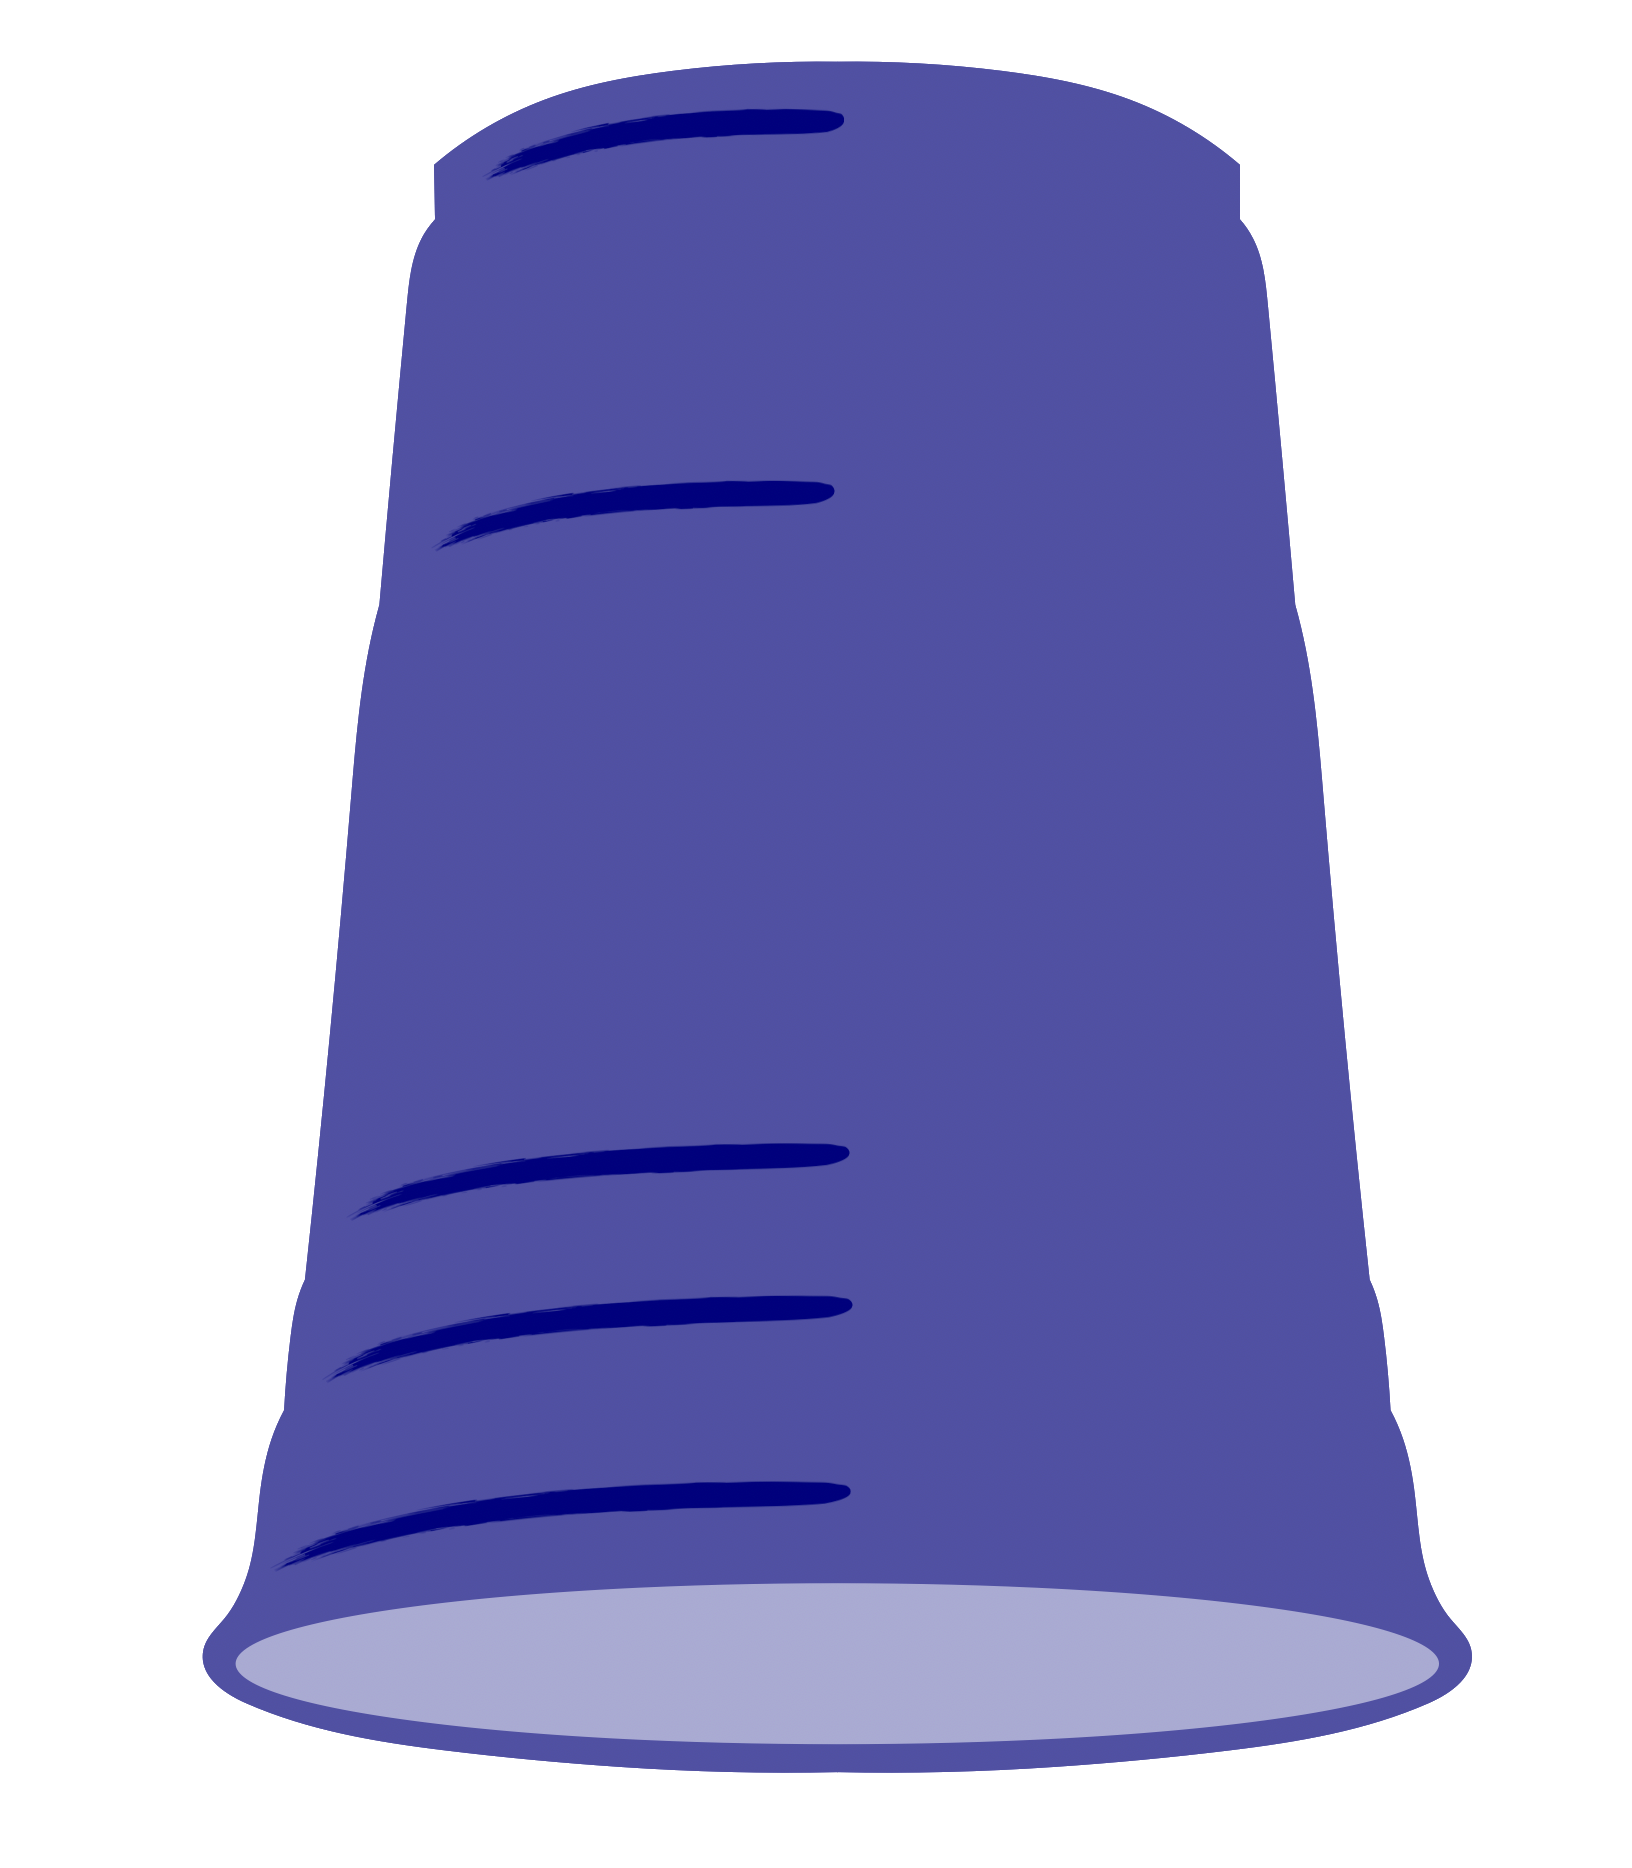
\includegraphics[width=2cm]{cup_up.png}};

				\fill[mid] (0, 4) circle (1);
				\begin{scope}
					\clip (0, 4) circle (1);
					\draw[color=dark, line width=2] (1.1, 4.3) arc[x radius=1.1, y radius=0.2, start angle=0, end angle=180];
					\draw[color=dark, line width=2] (1.1, 3.7) arc[x radius=1.1, y radius=0.2, start angle=0, end angle=180];
				\end{scope}
				\node at (0, 10) {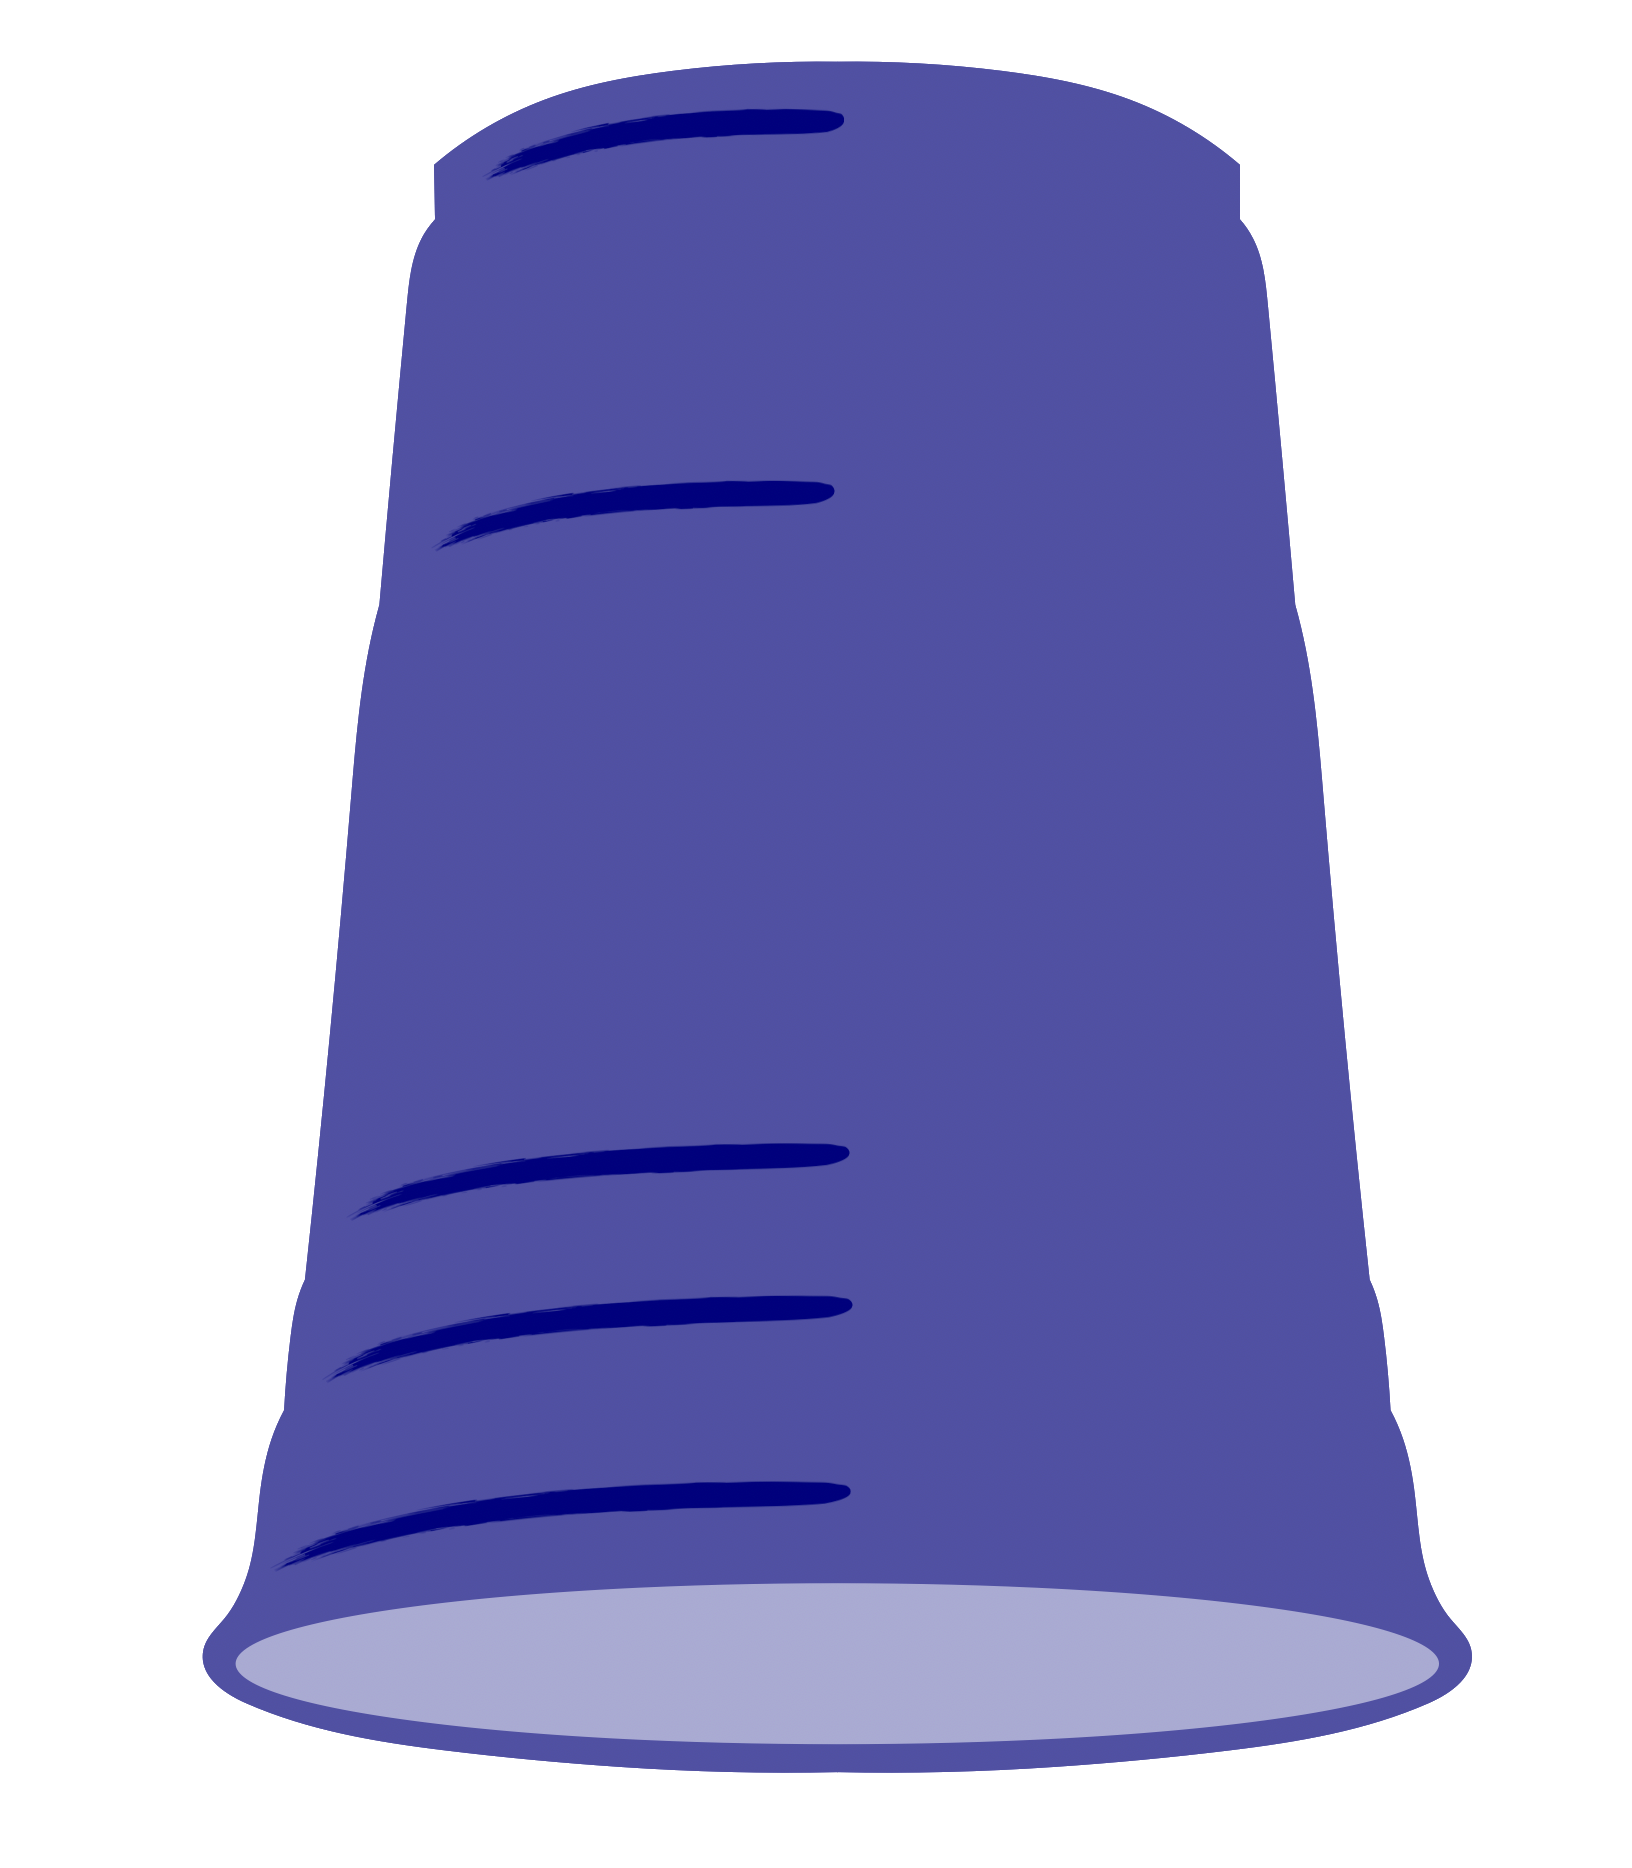
\includegraphics[width=2cm]{cup_up.png}};

				\fill[dark] (+10, 4) circle (1);
				\begin{scope}
					\clip (10, 4) circle (1);
					\draw[color=mid, line width=1] (10, 3) -- (10, 5);
					\draw[color=mid, line width=1] (10.25, 5) arc[x radius=0.3, y radius=1.1, start angle=90, end angle=-90];
					\draw[color=mid, line width=1] (9.75, 5) arc[x radius=0.3, y radius=1.1, start angle=90, end angle=270];
				\end{scope}
				\node at (+10, 10) {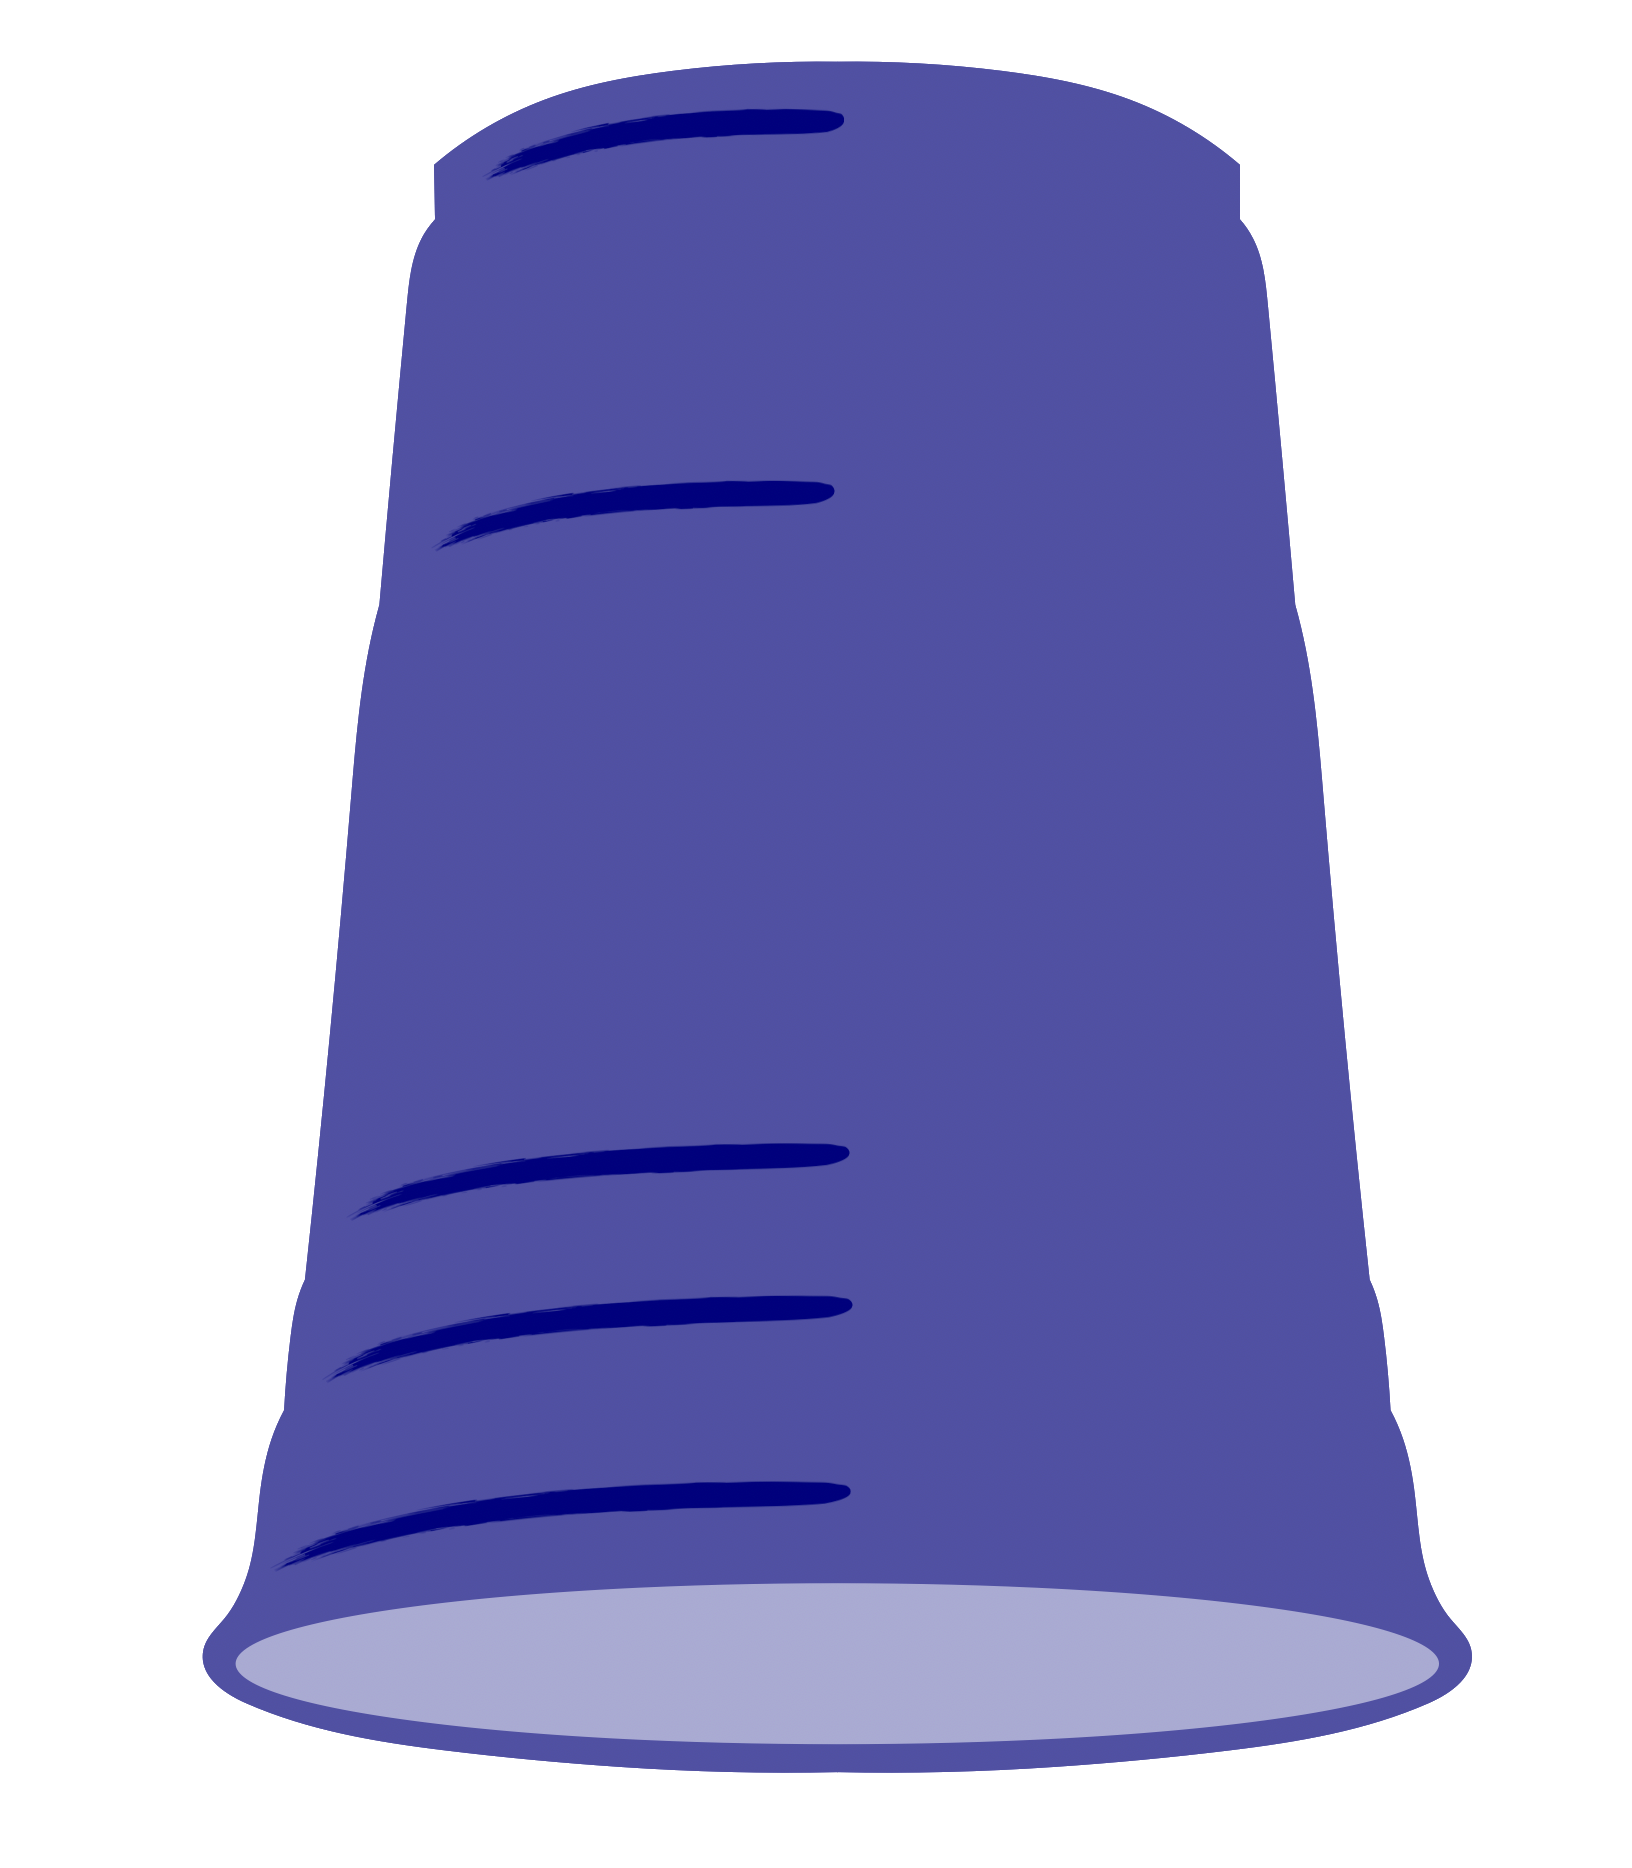
\includegraphics[width=2cm]{cup_up.png}};

			\end{scope}

			% Right
			\begin{scope}[shift={(0, 0)}]

				\draw[white] (-17, 0) rectangle (17, 15);

				\fill[dark] (-10, 4) circle (1);
				\node at (-10, 7) {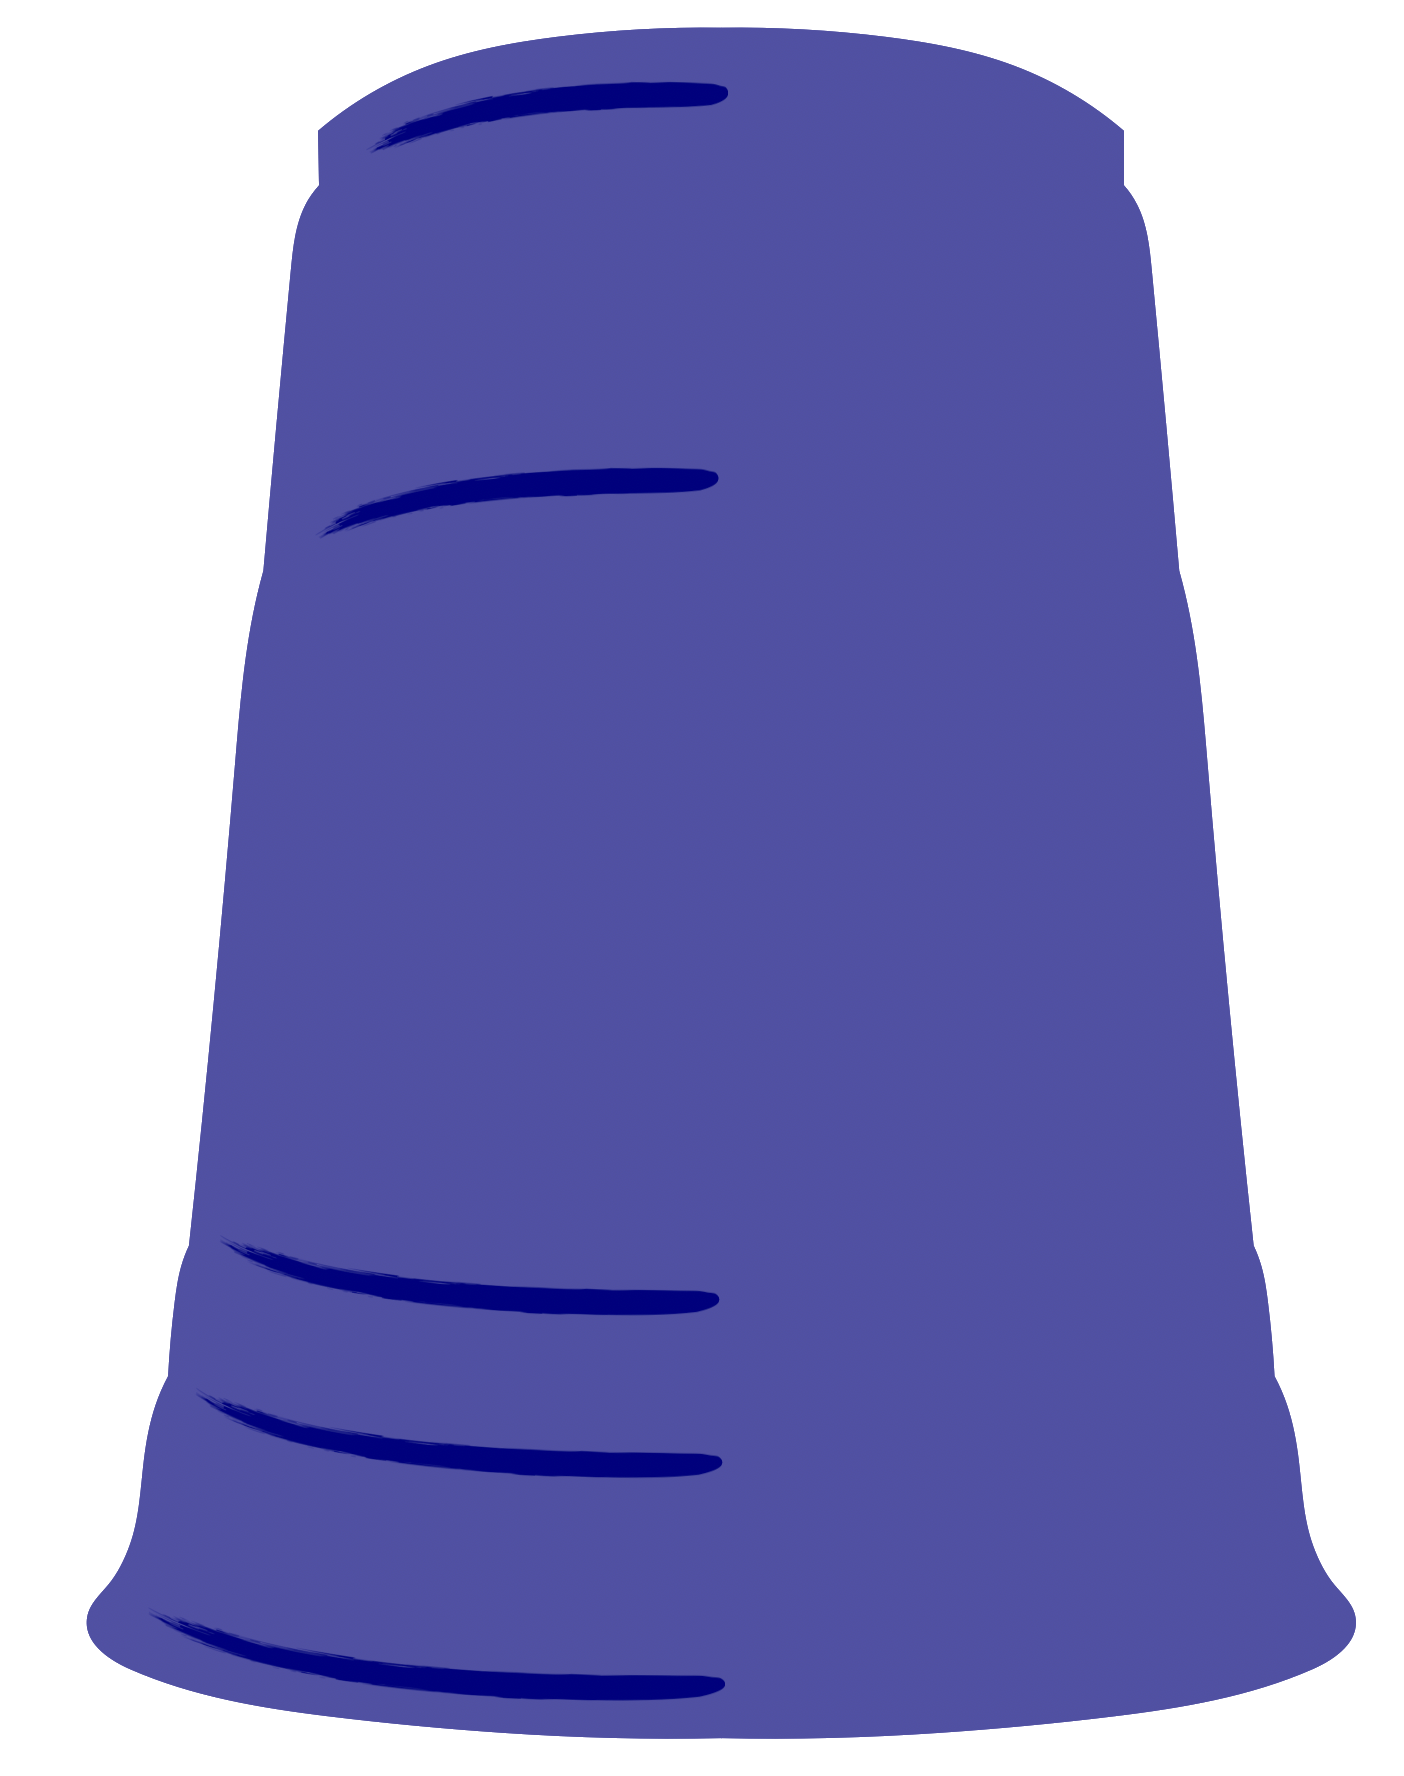
\includegraphics[width=2cm]{cup_down.png}};
				\begin{scope}[scale=0.7, shift={(-17, 3)}, rotate=-5]
					\fill[dark, rounded corners=3] (0, 0) rectangle (10, 6);
					\fill[black] (0, 0.5) rectangle (10, 3.5);
					\node[text=white, align=center, rotate=-5] at (5, 5.2) { \small \textsf{HELLO} };
					\node[text=white, align=center, rotate=-5] at (5, 4.1) { \tiny \textsf{my name is} };
					\node[text=white, align=center, rotate=0] at (5.25, 2) { \large \textsl{Group 1} };
				\end{scope}

				\fill[dark] (0, 4) circle (1);
				\node at (0, 7) {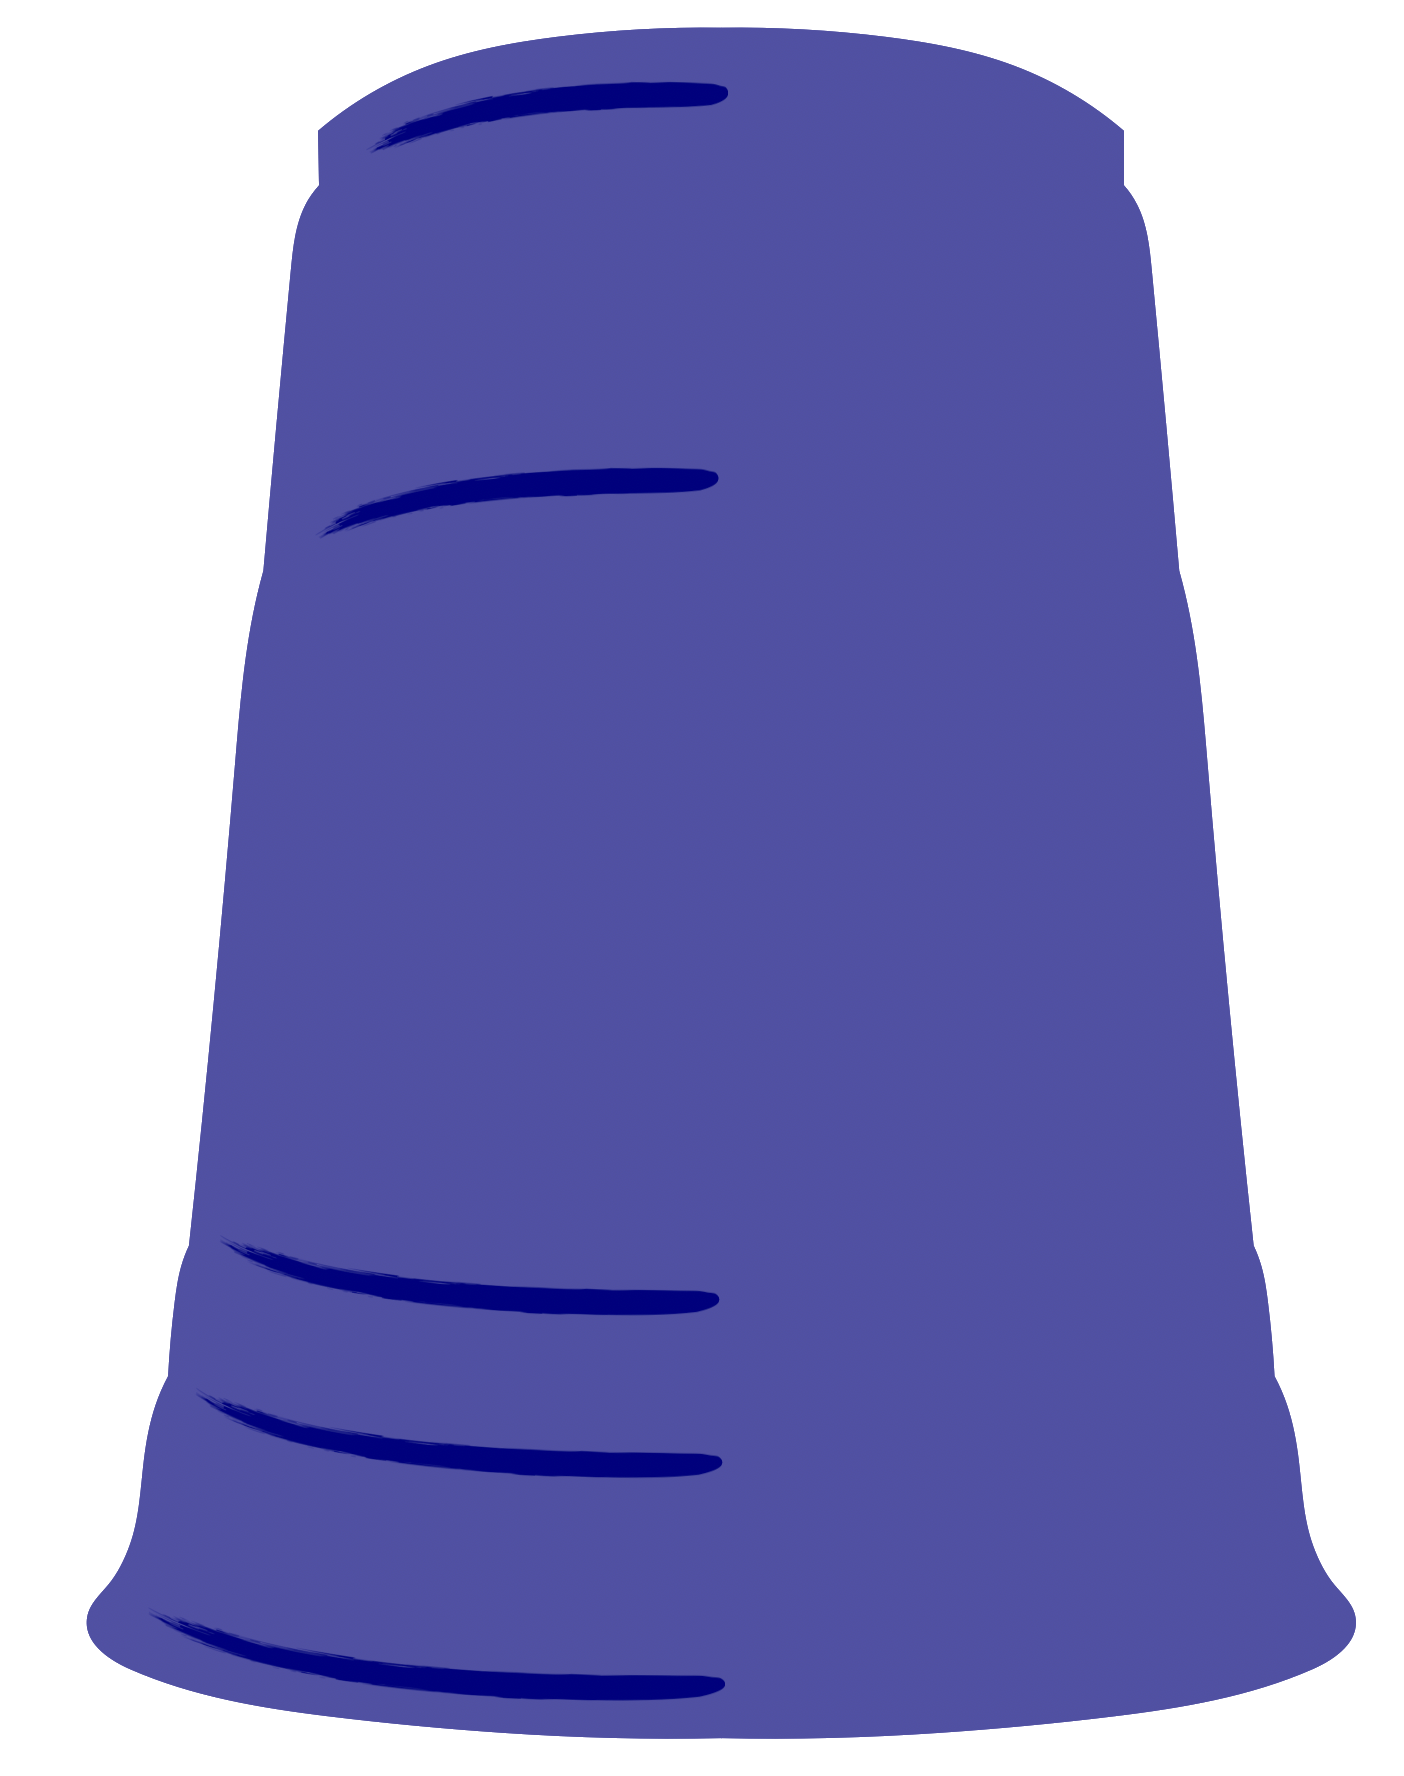
\includegraphics[width=2cm]{cup_down.png}};
				\begin{scope}[scale=0.7, shift={(-2, 3)}, rotate=10]
					\fill[dark, rounded corners=3] (0, 0) rectangle (10, 6);
					\fill[black] (0, 0.5) rectangle (10, 3.5);
					\node[text=white, align=center, rotate=10] at (5, 5.2) { \small \textsf{HELLO} };
					\node[text=white, align=center, rotate=10] at (5, 4.1) { \tiny \textsf{my name is } };
					\node[text=white, align=center, rotate=7] at (5.25, 2) { \large \textsl{Group 2} };
				\end{scope}

				\fill[dark] (+10, 4) circle (1);
				\node at (+10, 7) {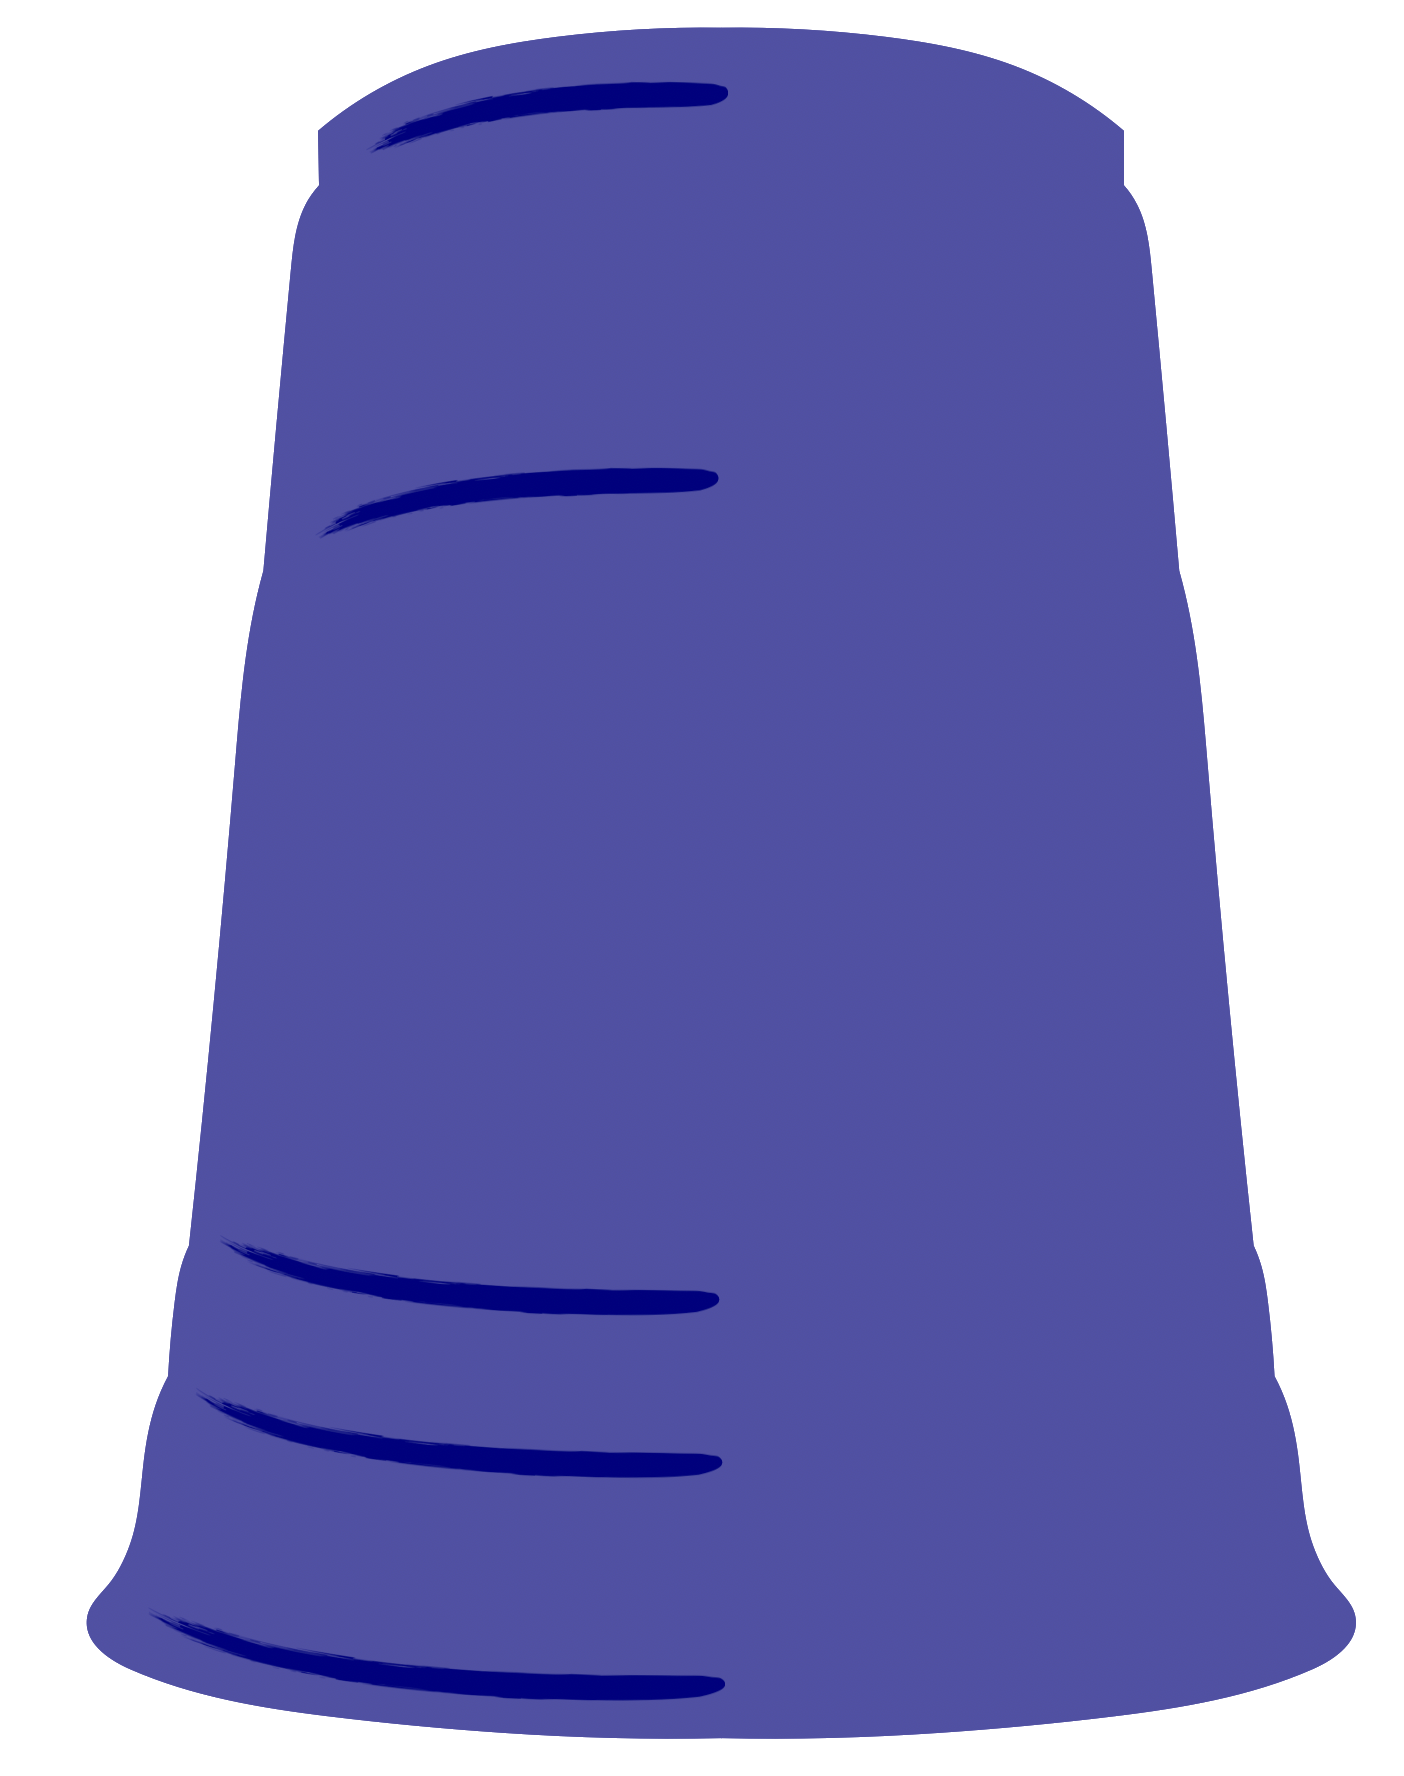
\includegraphics[width=2cm]{cup_down.png}};
				\begin{scope}[scale=0.7, shift={(12, 3)}, rotate=1]
					\fill[dark, rounded corners=3] (0, 0) rectangle (10, 6);
					\fill[black] (0, 0.5) rectangle (10, 3.5);
					\node[text=white, align=center, rotate=1] at (5, 5.2) { \small \textsf{HELLO} };
					\node[text=white, align=center, rotate=1] at (5, 4.1) { \tiny \textsf{my name is } };
					\node[text=white, align=center, rotate=1] at (5.25, 2) { \large \textsl{Group 3} };
				\end{scope}
			\end{scope}
		\end{tikzpicture}
	\end{adjustbox}
\end{frame}

\begin{frame}{Exchangeability \parencite{definettiTheoryProbability1974}\footnote{figures adapted from \href{https://betanalpha.github.io/assets/case_studies/hierarchical_modeling.html}{Michael Betancourt (CC-BY-SA-4.0)}.}}
	\begin{adjustbox}{max width=1.0\textwidth}
		\begin{tikzpicture}[scale=0.3, thick]


			\draw[white] (-17, -3) rectangle (17, 15);

			\fill[dark] (-10, 4) circle (1);
			\node at (-10, 7) {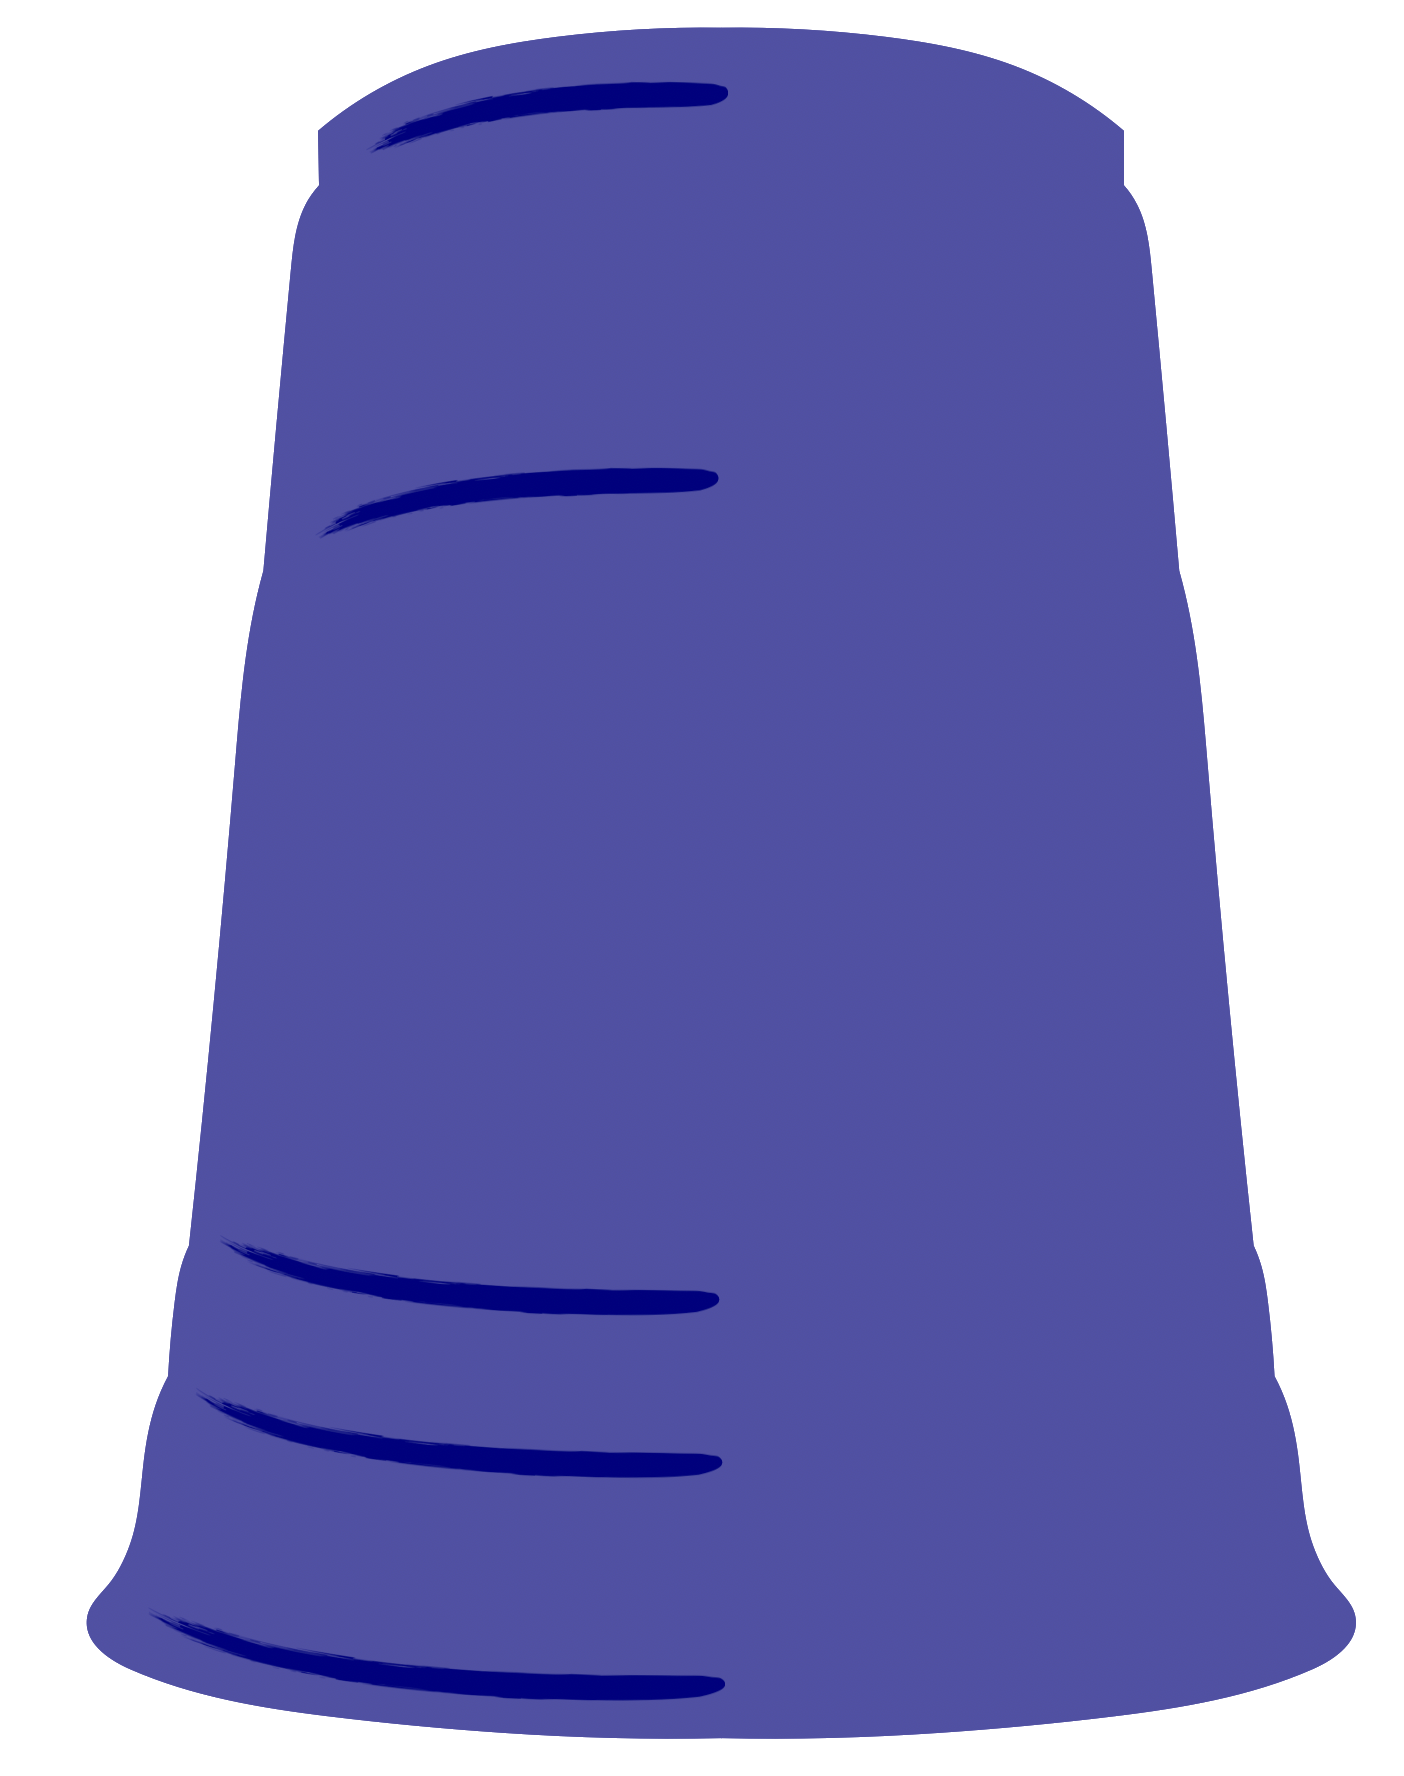
\includegraphics[width=2cm]{cup_down.png}};

			% Left
			\begin{scope}[scale=0.7, shift={(-17, 3)}, rotate=-5]
				\fill[dark, rounded corners=3] (0, 0) rectangle (10, 6);
				\fill[black] (0, 0.5) rectangle (10, 3.5);
				\node[text=white, align=center, rotate=-5] at (5, 5.2) { \small \textsf{HELLO} };
				\node[text=white, align=center, rotate=-5] at (5, 4.1) { \tiny \textsf{my name is } };
				\node[text=white, align=center, rotate=0] at (5.25, 2) { \large \textsl{Group 1} };
			\end{scope}

			\fill[dark] (0, 4) circle (1);
			\node at (0, 7) {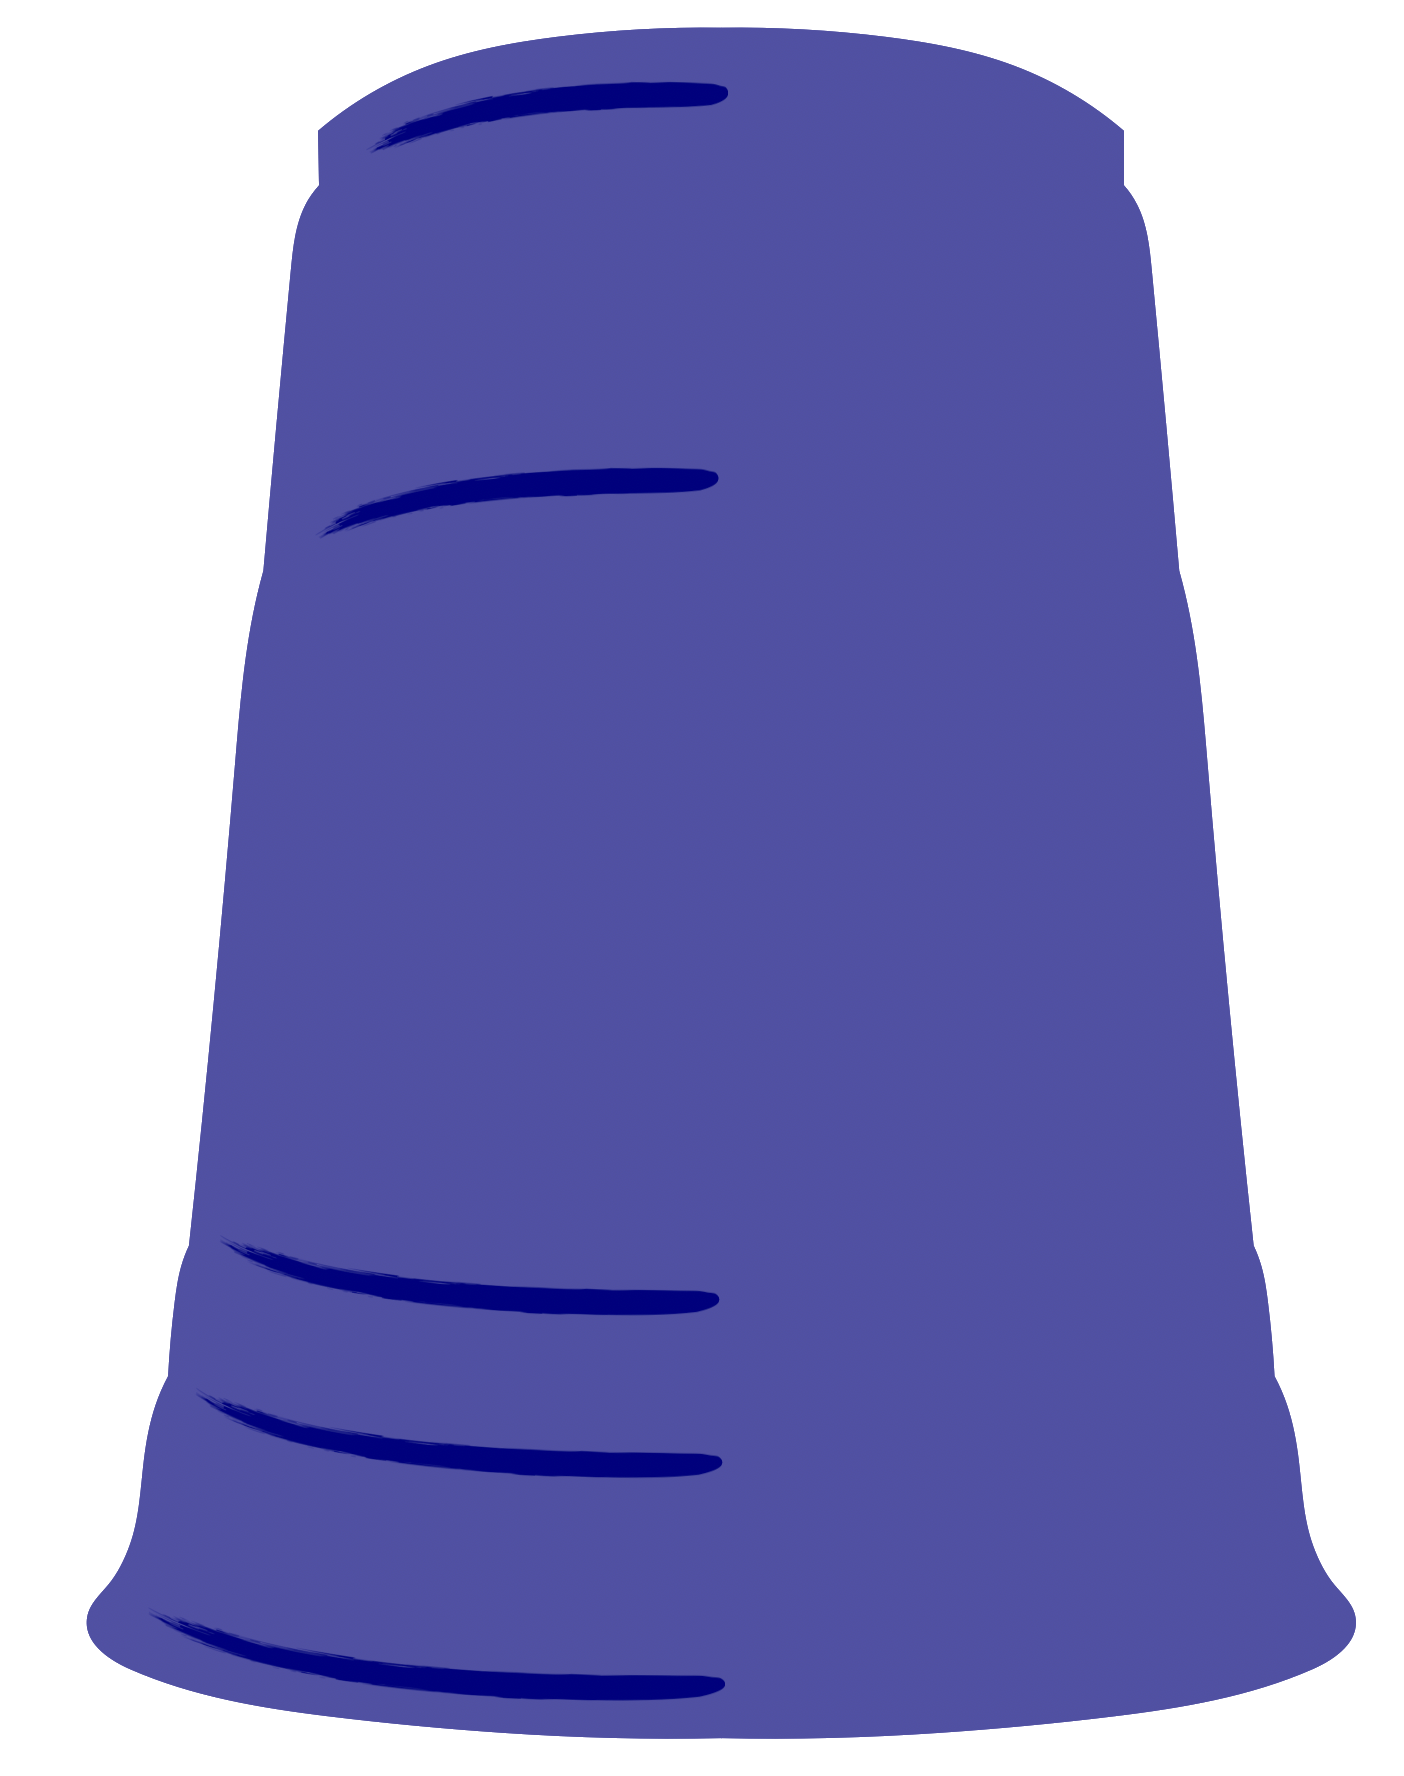
\includegraphics[width=2cm]{cup_down.png}};

			\begin{scope}[scale=0.7, shift={(-2, 3)}, rotate=10]
				\fill[dark, rounded corners=3] (0, 0) rectangle (10, 6);
				\fill[black] (0, 0.5) rectangle (10, 3.5);
				\node[text=white, align=center, rotate=10] at (5, 5.2) { \small \textsf{HELLO} };
				\node[text=white, align=center, rotate=10] at (5, 4.1) { \tiny \textsf{my name is } };
				\node[text=white, align=center, rotate=7] at (5.25, 2) { \large \textsl{Group 2} };
			\end{scope}

			\fill[dark] (+10, 4) circle (1);
			\node at (+10, 7) {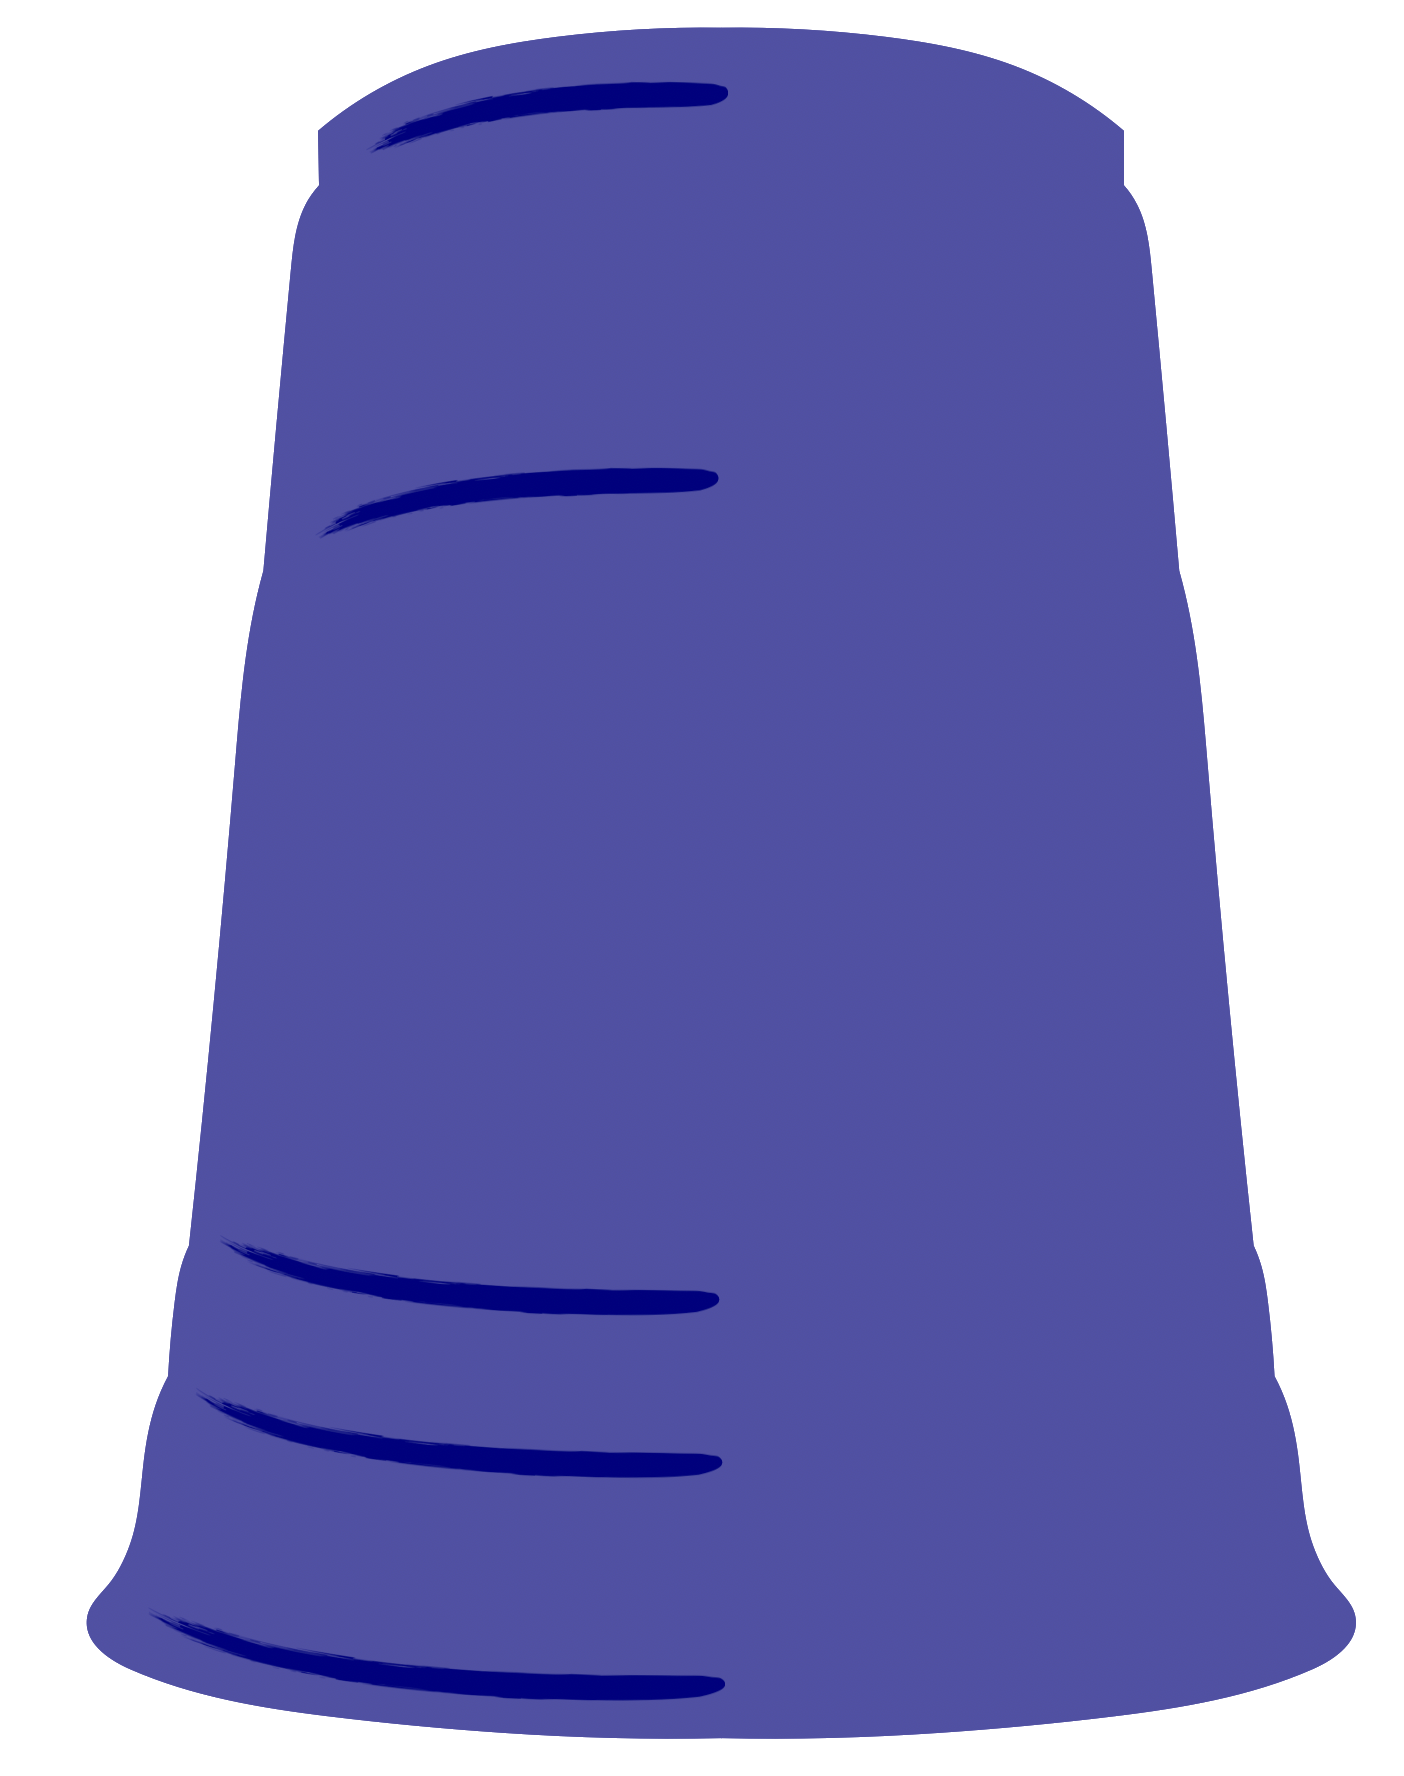
\includegraphics[width=2cm]{cup_down.png}};

			\begin{scope}[scale=0.7, shift={(12, 3)}, rotate=1]
				\fill[dark, rounded corners=3] (0, 0) rectangle (10, 6);
				\fill[black] (0, 0.5) rectangle (10, 3.5);
				\node[text=white, align=center, rotate=1] at (5, 5.2) { \small \textsf{HELLO} };
				\node[text=white, align=center, rotate=1] at (5, 4.1) { \tiny \textsf{my name is } };
				\node[text=white, align=center, rotate=1] at (5.25, 2) { \large \textsl{Group 3} };
			\end{scope}

			\pgfmathsetmacro{\r}{10}
			\pgfmathsetmacro{\start}{160}
			\pgfmathsetmacro{\stop}{20}

			\draw[dark, <->, >=stealth] ({0 + \r * cos(\start)}, {8 + \r * sin(\start)})
			arc[x radius = \r, y radius = 3, start angle=\start, end angle= \stop];

			\pgfmathsetmacro{\r}{3}
			\pgfmathsetmacro{\start}{160}
			\pgfmathsetmacro{\stop}{20}

			\draw[dark, <->, >=stealth] ({-5 + \r * cos(\start)}, {10 + \r * sin(\start)})
			arc[x radius = \r, y radius = 0.75, start angle=\start, end angle= \stop];

			\draw[dark, <->, >=stealth] ({5 + \r * cos(\start)}, {10 + \r * sin(\start)})
			arc[x radius = \r, y radius = 0.75, start angle=\start, end angle= \stop];

			% Right
			\begin{scope}[shift={(36, 0)}]

				\draw[white] (-17, -3) rectangle (17, 15);

				\fill[dark] (-10, 4) circle (1);
				\node at (-10, 7) {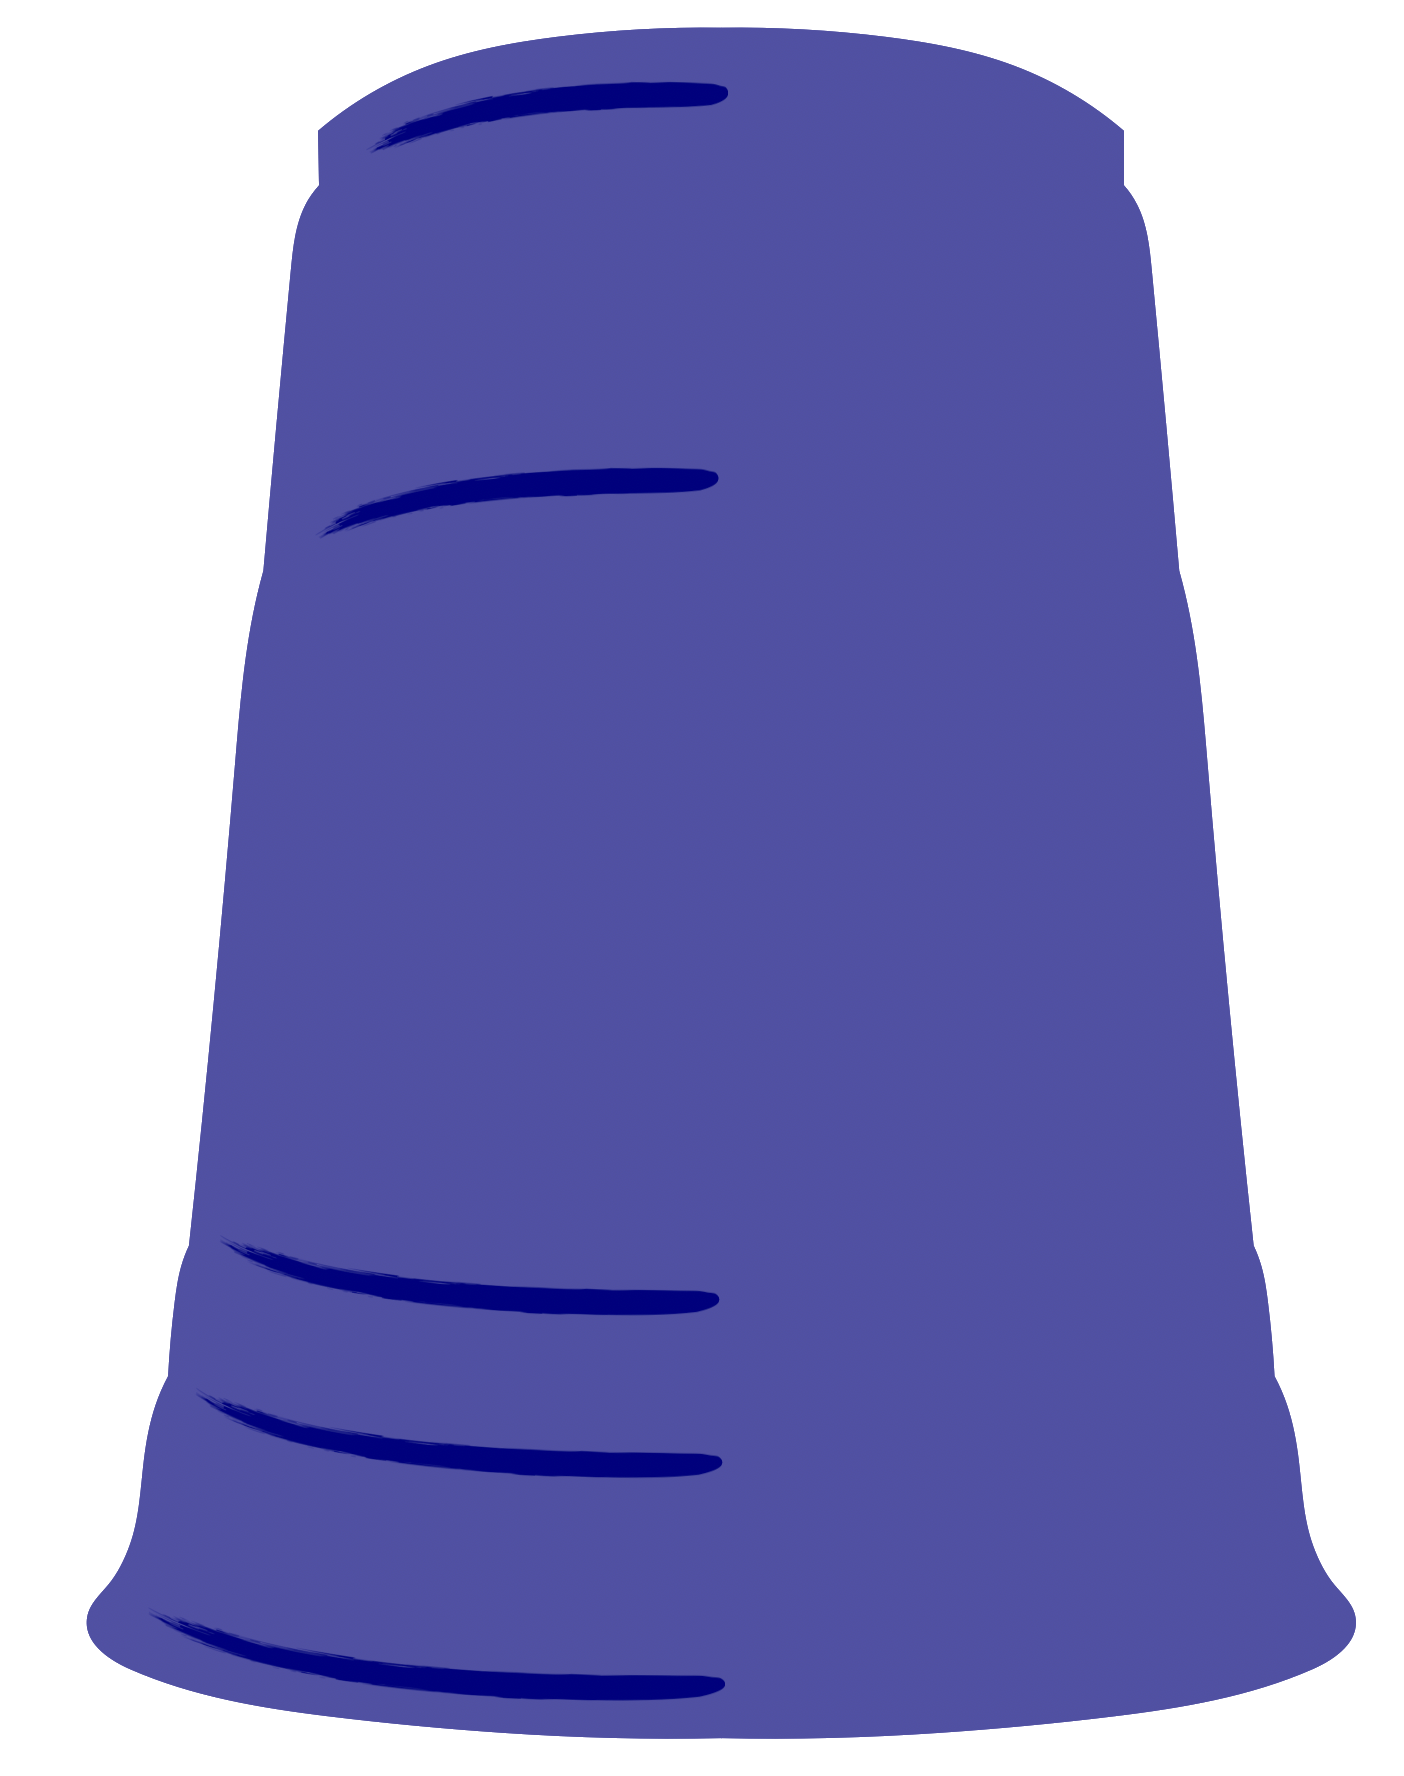
\includegraphics[width=2cm]{cup_down.png}};

				\begin{scope}[scale=0.7, shift={(-17, 3)}, rotate=-5]
					\fill[dark, rounded corners=3] (0, 0) rectangle (10, 6);
					\fill[black] (0, 0.5) rectangle (10, 3.5);
					\node[text=white, align=center, rotate=-5] at (5, 5.2) { \small \textsf{HELLO} };
					\node[text=white, align=center, rotate=-5] at (5, 4.1) { \tiny \textsf{my name is } };
					\node[text=white, align=center, rotate=0] at (5.25, 2) { \large \textsl{Group 3} };
				\end{scope}

				\fill[dark] (0, 4) circle (1);
				\node at (0, 7) {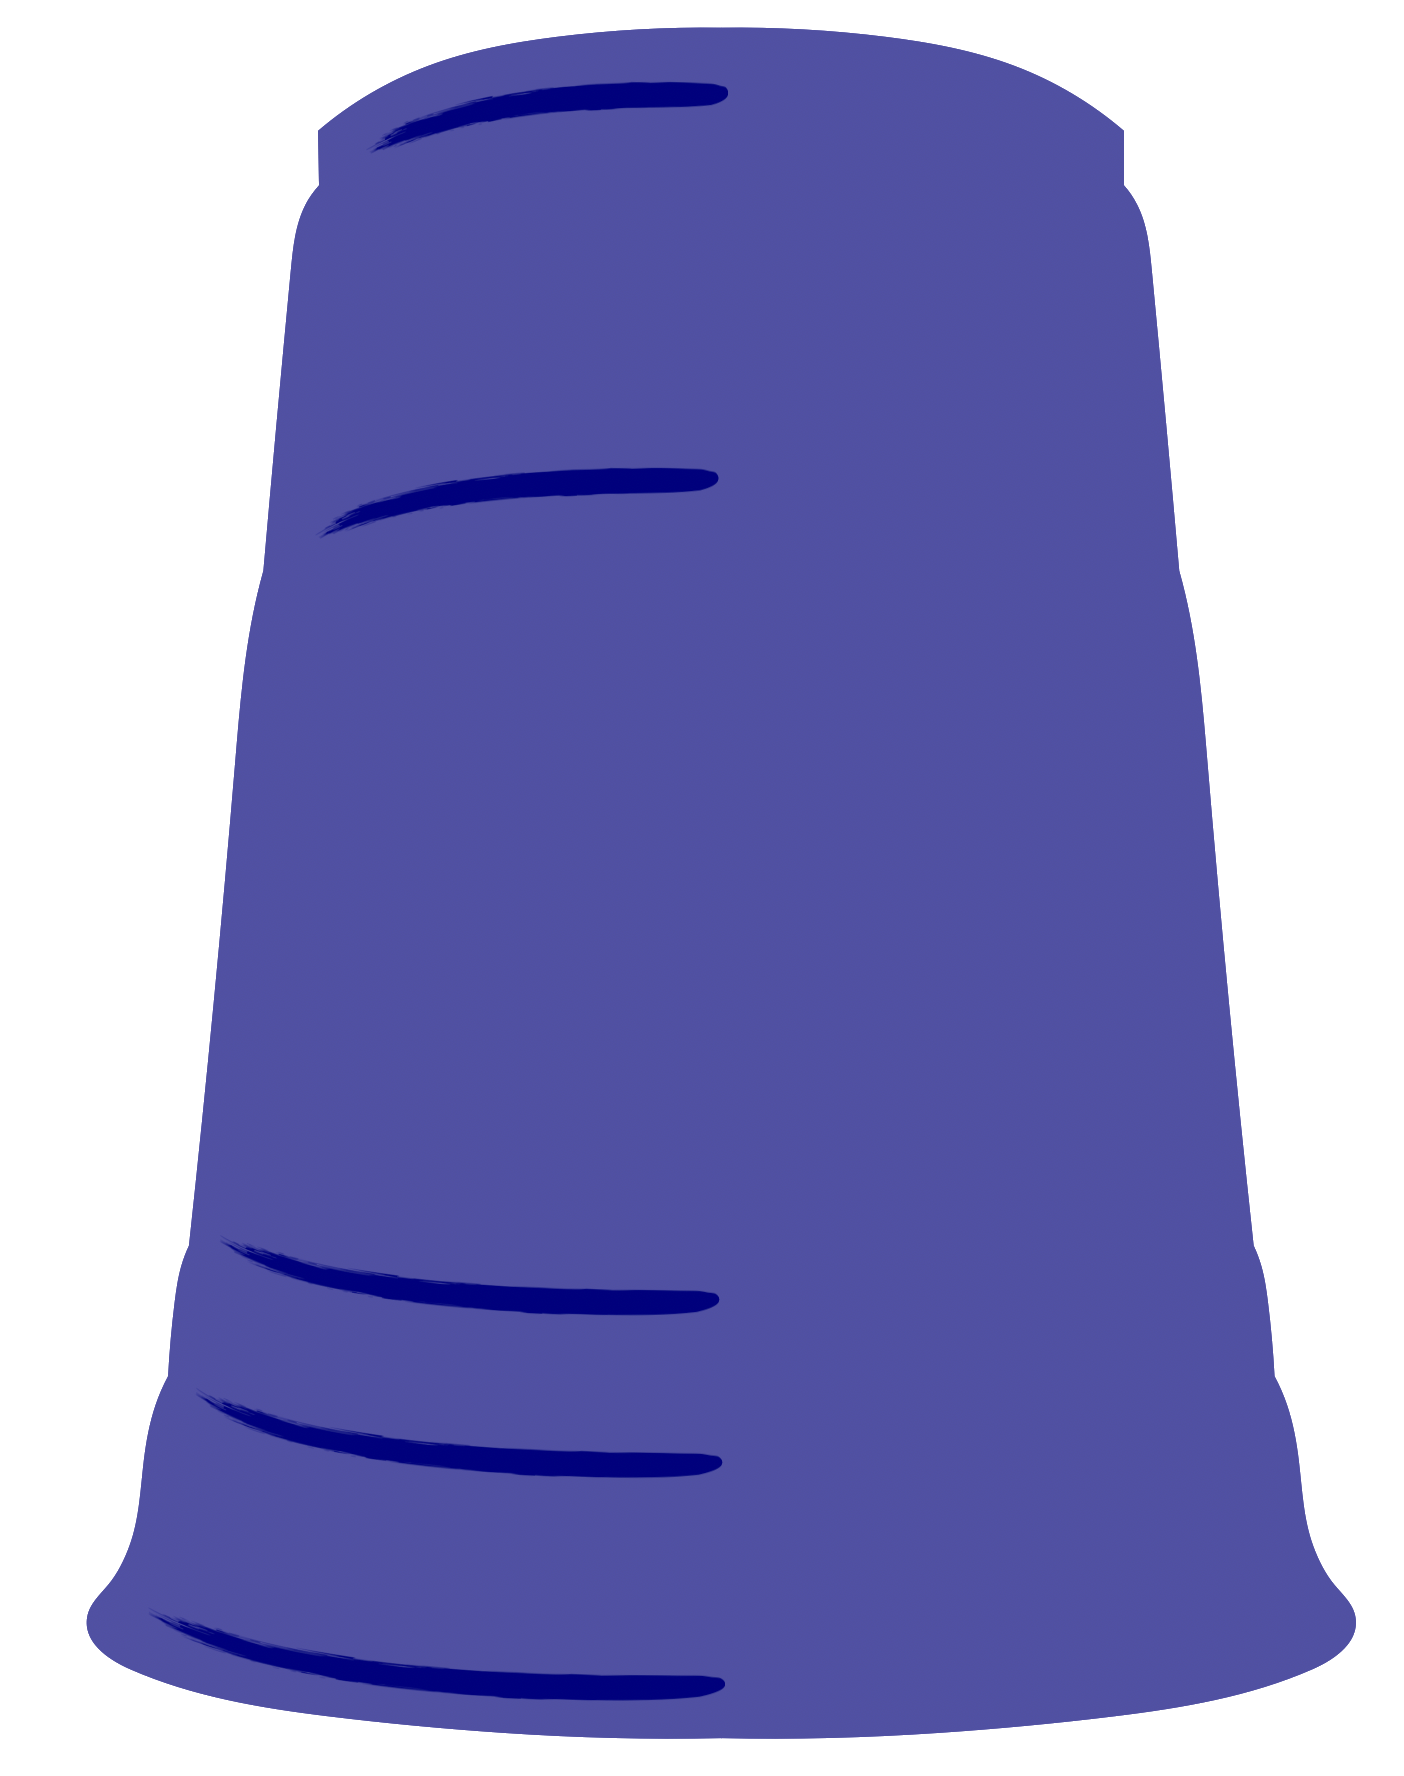
\includegraphics[width=2cm]{cup_down.png}};

				\begin{scope}[scale=0.7, shift={(-2, 3)}, rotate=10]
					\fill[dark, rounded corners=3] (0, 0) rectangle (10, 6);
					\fill[black] (0, 0.5) rectangle (10, 3.5);
					\node[text=white, align=center, rotate=10] at (5, 5.2) { \small \textsf{HELLO} };
					\node[text=white, align=center, rotate=10] at (5, 4.1) { \tiny \textsf{my name is } };
					\node[text=white, align=center, rotate=7] at (5.25, 2) { \large \textsl{Group 1} };
				\end{scope}

				\fill[dark] (+10, 4) circle (1);
				\node at (+10, 7) {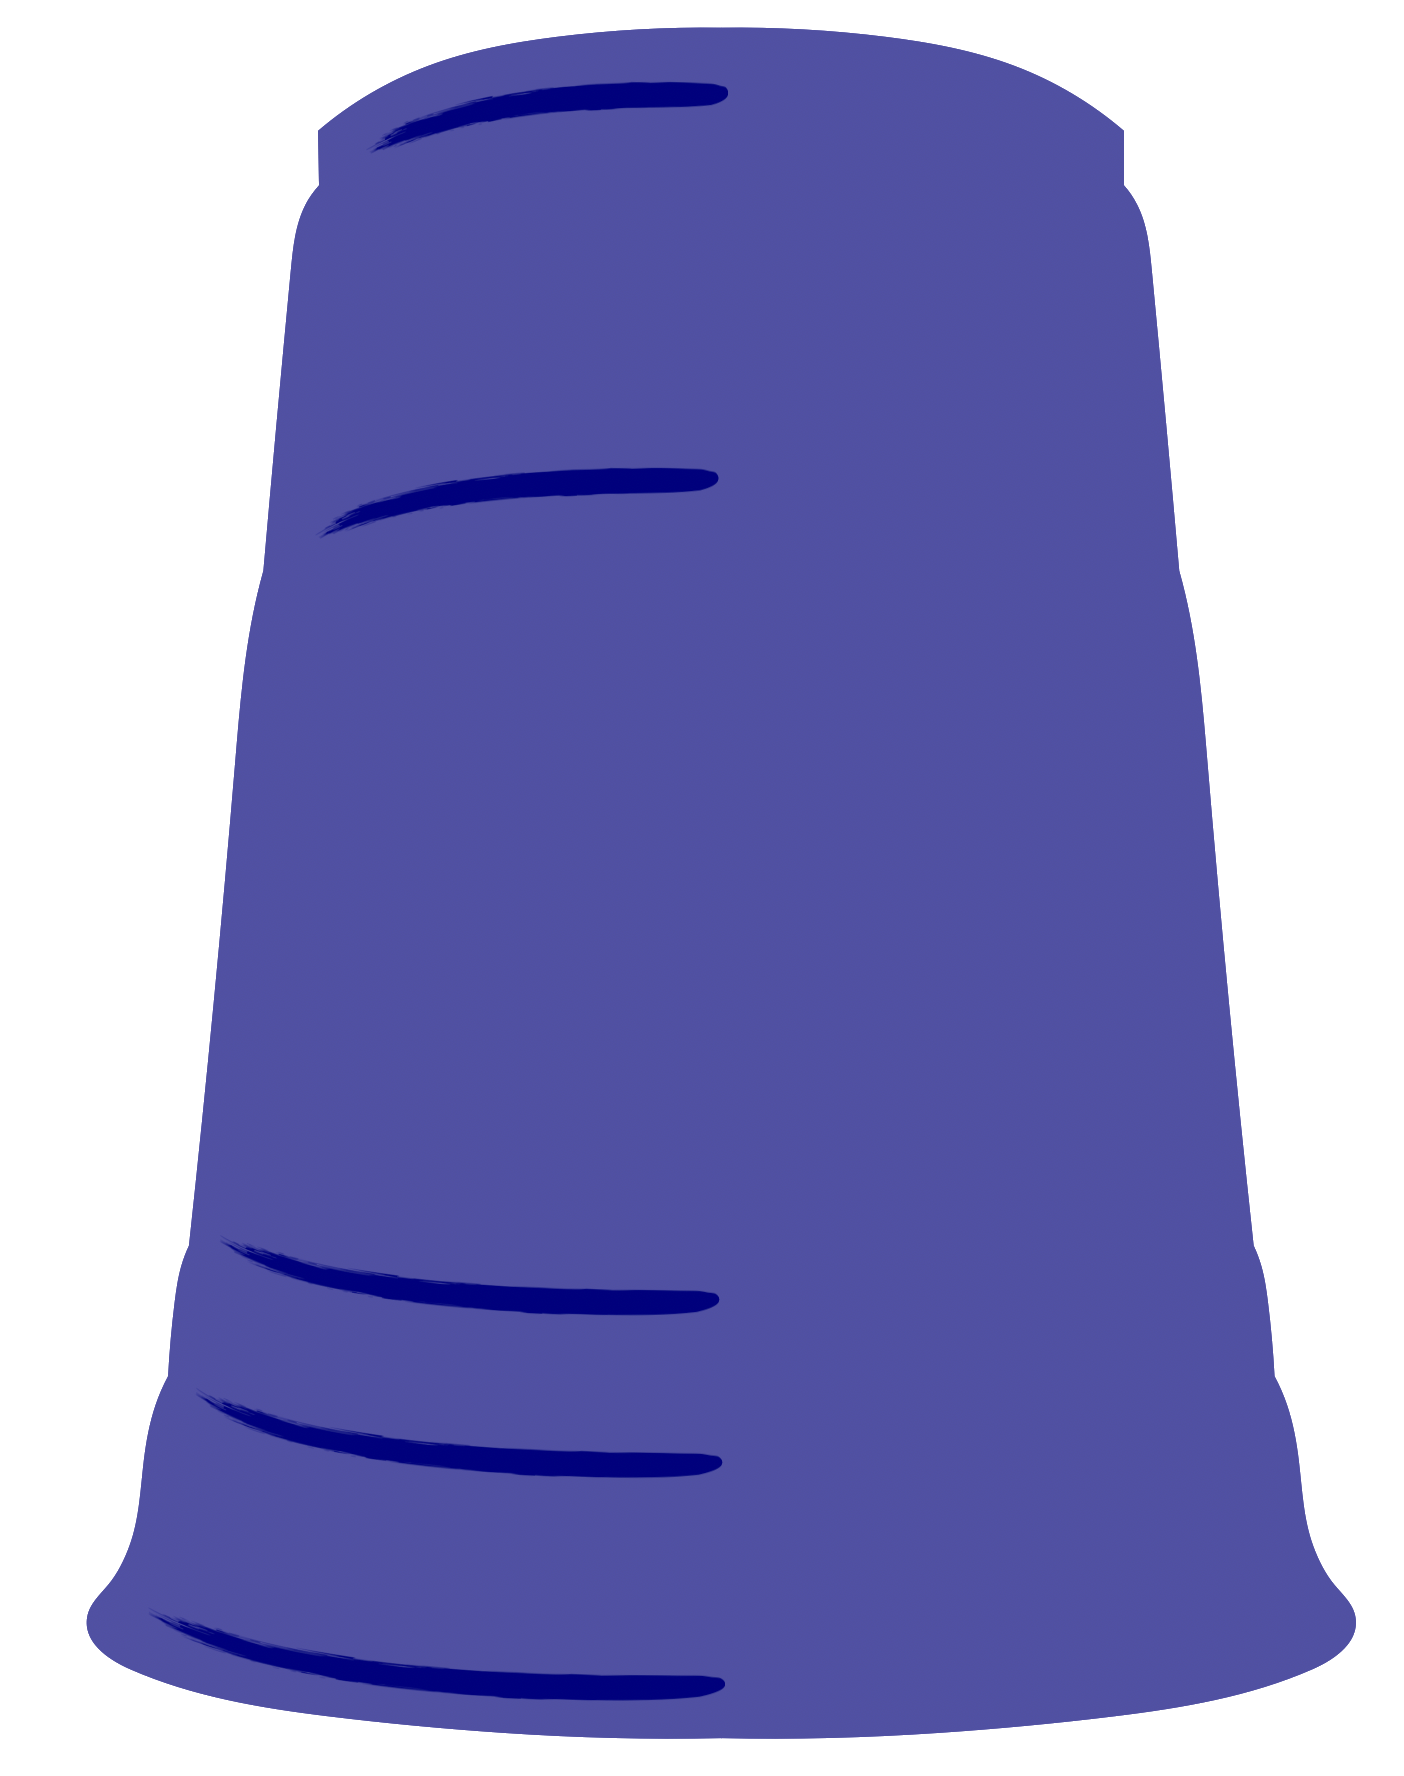
\includegraphics[width=2cm]{cup_down.png}};

				\begin{scope}[scale=0.7, shift={(12, 3)}, rotate=1]
					\fill[dark, rounded corners=3] (0, 0) rectangle (10, 6);
					\fill[black] (0, 0.5) rectangle (10, 3.5);
					\node[text=white, align=center, rotate=1] at (5, 5.2) { \small \textsf{HELLO} };
					\node[text=white, align=center, rotate=1] at (5, 4.1) { \tiny \textsf{my name is } };
					\node[text=white, align=center, rotate=1] at (5.25, 2) { \large \textsl{Group 2} };
				\end{scope}

				\draw[light, <->, >=stealth, line width=4]
				(-8, 6.5) .. controls (-7, 7.5) and (-6.5, 8.25) ..
				(-4.5, 8.5) .. controls (-2.5, 8.75) and (-1, 8.5) .. (0, 7);
				\draw[dark, <->, >=stealth, line width=2]
				(-7.85, 6.65) .. controls (-7, 7.5) and (-6.5, 8.25) ..
				(-4.5, 8.5) .. controls (-2.5, 8.75) and (-1, 8.5) .. (-0.15, 7.15);

				\draw[light, <->, >=stealth, line width=4]
				(3, 7.5) .. controls (4, 9) and (6.25, 9.75) ..
				(8.25, 9.5) .. controls (10.25, 9.25) and (11, 8.75) .. (12, 6.75);
				\draw[dark, <->, >=stealth, line width=2]
				(3.15, 7.65) .. controls (4, 9) and (6.25, 9.75) ..
				(8.25, 9.5) .. controls (10.25, 9.25) and (11, 8.75) .. (11.9, 6.9);

				\draw[light, <->, >=stealth, line width=4]
				(-8, 1.5) .. controls (-7, -1.5) and (2, -1.25) ..
				(4, -1) .. controls (6, -0.75) and (11, -0.5) .. (12, 1.5);
				\draw[dark, <->, >=stealth, line width=2]
				(-7.925, 1.25) .. controls (-7, -1.5) and (2, -1.25) ..
				(4, -1) .. controls (6, -0.75) and (11, -0.5) .. (11.9, 1.3);

			\end{scope}

		\end{tikzpicture}
	\end{adjustbox}
\end{frame}

\subsection{Hyperprior}
\begin{frame}{Hyperprior}
	In hierarchical models, we have a hyperprior,
	which is a prior's prior:
	$$
		\begin{aligned}
			\mathbf{y}          & \sim \text{Normal}(10, \boldsymbol{\theta}) \\
			\boldsymbol{\theta} & \sim \text{Normal}(0, \phi)                 \\
			\phi                & \sim \text{Exponential(1)}
		\end{aligned}
	$$
	Here $\mathbf{y}$ is a variable of interest that belongs to distinct groups.
	$\boldsymbol{\theta}$, a prior for $\mathbf{y}$,
	is a vector of group-leve parameters with their own prior
	(which becomes a hiperprior) $\phi$.
\end{frame}

\subsection{Frequentist versus Bayesian Approaches}
\begin{frame}{Frequentist versus Bayesian Approaches}
	There are also hierarchical models in frequentist statistics.
	They are mainly available in the \texttt{lme4} package \parencite{lme4},
	and also in \texttt{MixedModels.jl} (TODO: CITATION).
	\begin{vfilleditems}
		\item \textbf{optimization of the likelihood function} versus \textbf{posterior approximation via MCMC}.
		Almost always lead to convergence failure for models that are not extremely simple.
		\item \textbf{frequentist hierarchical models do not compute $p$-values for the group-level effects}\footnote{
			see \href{https://stat.ethz.ch/pipermail/r-help/2006-May/094765.html}
			{Douglas Bates, creator of the \texttt{lme4} package explanation}.}.
		This is due to the underlying assumptions of the approximations that frequentist
		statistics has to to do in order to calculate the group-level effects $p$-values.
		The main one being that the groups must be balanced.
		In other words, the groups must be homogeneous in size.
		Hence, any unbalance in group compositions results in pathological $p$-values
		that should not be trusted.
	\end{vfilleditems}
\end{frame}

\begin{frame}{Frequentist versus Bayesian Approaches}
	To sum up, \textbf{frequentist approach for hierarchical models is not robust}
	in both the \textbf{inference process}
	(\textbf{convergence flaws} during the maximum likelihood estimation),
	and also in the \textbf{results} from the inference process
	(do not provide $p$-values due to
	\textbf{strong assumptions that are almost always violated}).
\end{frame}

\subsection{Approaches to Hierarchical Modeling}
\begin{frame}{Approaches to Hierarchical Modeling}
	\begin{vfilleditems}
		\item \textbf{Varying-intercept} model:
		One group-level intercept besides the population-level
		intercept and coefficients.
		\item \textbf{Varying-slope} model:
		One or more group-level coefficient(s) besides the population-level
		intercept and coefficients.
		\item \textbf{Varying-intercept-slope} model:
		One group-level intercept and one or more group-level coefficient(s) besides the population-level
		intercept and coefficients.
		\item \textbf{Correlated varying-intercept-slope} model:
		One group-level intercept and one or more group-level coefficient(s) besides the population-level
		intercept and coefficients.
		Here the group-level intercept and coefficients priors
		are \textbf{sampled from the same multivariate distribution}.
	\end{vfilleditems}
\end{frame}

\begin{frame}{Mathematical Specification of Hierarchical Models}
	We have $N$ observations organized in $J$ groups with $K$ independent variables.
	\vfill
	Here we insert a column filled with $1$s in the data matrix $\mathbf{X}$.
	\vfill
	Mathematically, this makes the column behave like an ``identity'' variable
	(because the number $1$ in the multiplication operation $1 \cdot \beta$ is the identity element.
	It maps $x \to x$ keeping the value of $x$ intact) and, consequently,
	we can interpret the column's coefficient as the model's intercept.
\end{frame}

\begin{frame}{Mathematical Specification of Hierarchical Models}
	Hence, we have as a data matrix:
	$$
		\mathbf{X} =
		\begin{bmatrix}
			1      & x_{11} & x_{12} & \cdots & x_{1K} \\
			1      & x_{21} & x_{22} & \cdots & x_{2K} \\
			\vdots & \cdots & \cdots & \ddots & \vdots \\
			1      & x_{N1} & x_{N2} & \cdots & x_{NK}
		\end{bmatrix}
	$$
\end{frame}

\begin{frame}{Mathematical Specification -- Varying-Intercept Model}
	This example is for linear regression:
	$$
		\begin{aligned}
			\mathbf{y}         & \sim \text{Normal}\left( \alpha + \alpha_j + \mathbf{X} \cdot \boldsymbol{\beta}, \sigma \right) \\
			\alpha             & \sim \text{Normal}(\mu_\alpha, \sigma_\alpha)                                                    \\
			\alpha_j           & \sim \text{Normal}(0, \tau)                                                                      \\
			\boldsymbol{\beta} & \sim \text{Normal}(\mu_{\boldsymbol{\beta}}, \sigma_{\boldsymbol{\beta}})                        \\
			\tau               & \sim \text{Cauchy}^+(0, \psi_{\alpha})                                                           \\
			\sigma             & \sim \text{Exponential}(\lambda_\sigma)
		\end{aligned}
	$$
\end{frame}

\begin{frame}{Mathematical Specification -- Varying-Intercept Model}
	If you need to extend to more than one group,
	such as $J_1, J_2, \dots$:
	$$
		\begin{aligned}
			\mathbf{y}         & \sim \text{Normal}(\alpha + \alpha_{j1} + \alpha_{j2} + \mathbf{X} \boldsymbol{\beta}, \sigma) \\
			\alpha             & \sim \text{Normal}(\mu_\alpha, \sigma_\alpha)                                                  \\
			\alpha_{j1}        & \sim \text{Normal}(0, \tau_{\alpha j1})                                                        \\
			\alpha_{j2}        & \sim \text{Normal}(0, \tau_{\alpha j2})                                                        \\
			\boldsymbol{\beta} & \sim \text{Normal}(\mu_{\boldsymbol{\beta}}, \sigma_{\boldsymbol{\beta}})                      \\
			\tau_{\alpha j1}   & \sim \text{Cauchy}^+(0, \psi_{\alpha j1})                                                      \\
			\tau_{\alpha j2}   & \sim \text{Cauchy}^+(0, \psi_{\alpha j2})                                                      \\
			\sigma             & \sim \text{Exponential}(\lambda_\sigma)
		\end{aligned}
	$$
\end{frame}

\begin{frame}{Mathematical Specification -- Varying-Slope Model}
	This example is for linear regression:
	$$
		\begin{aligned}
			\mathbf{y}           & \sim \text{Normal}\left( \alpha + \mathbf{X} \cdot \boldsymbol{\beta}_j \cdot \boldsymbol{\tau}, \sigma \right) \\
			\alpha               & \sim \text{Normal}(\mu_\alpha, \sigma_\alpha)                                                                   \\
			\boldsymbol{\beta}_j & \sim \text{Normal}(\mu_{\boldsymbol{\beta}}, \sigma_{\boldsymbol{\beta}})                                       \\
			\boldsymbol{\tau}    & \sim \text{Cauchy}^+(0, \psi_{\beta})                                                                           \\
			\sigma               & \sim \text{Exponential}(\lambda_\sigma)
		\end{aligned}
	$$
	$\boldsymbol{\tau}$ is a vector of priors for the group-level coefficients'
	standard deviation.
\end{frame}

\begin{frame}{Mathematical Specification -- Varying-Slope Model}
	If you need to extend to more than one group,
	such as $J_1, J_2, \dots$:
	$$
		\begin{aligned}
			\mathbf{y}                   & \sim \text{Normal}(\alpha + \mathbf{X} \boldsymbol{\beta}_{j1} \cdot \boldsymbol{\tau}_{j1} + \mathbf{X} \boldsymbol{\beta}_{j2} \cdot \boldsymbol{\tau}_{j2}, \sigma) \\
			\alpha                       & \sim \text{Normal}(\mu_\alpha, \sigma_\alpha)                                                                                                                          \\
			\boldsymbol{\beta}_{j1}      & \sim \text{Normal}(\mu_{\boldsymbol{\beta j1}}, \sigma_{\boldsymbol{\beta j1}})                                                                                        \\
			\boldsymbol{\beta}_{j2}      & \sim \text{Normal}(\mu_{\boldsymbol{\beta j2}}, \sigma_{\boldsymbol{\beta j2}})                                                                                        \\
			\boldsymbol{\tau}_{\beta j1} & \sim \text{Cauchy}^+(0, \psi_{\beta j1})                                                                                                                               \\
			\boldsymbol{\tau}_{\beta j2} & \sim \text{Cauchy}^+(0, \psi_{\beta j2})                                                                                                                               \\
			\sigma                       & \sim \text{Exponential}(\lambda_\sigma)
		\end{aligned}
	$$
\end{frame}

\begin{frame}{Mathematical Specification -- Varying-Intercept-Slope Model}
	This example is for linear regression:
	$$
		\begin{aligned}
			\mathbf{y}              & \sim \text{Normal}\left( \alpha + \alpha_j + \mathbf{X} \cdot \boldsymbol{\beta}_j \cdot \boldsymbol{\tau}_\beta, \sigma \right) \\
			\alpha                  & \sim \text{Normal}(\mu_\alpha, \sigma_\alpha)                                                                                    \\
			\alpha_j                & \sim \text{Normal}(0, \tau_\alpha)                                                                                               \\
			\boldsymbol{\beta}_j    & \sim \text{Normal}(\mu_{\boldsymbol{\beta}}, \sigma_{\boldsymbol{\beta}})                                                        \\
			\tau_\alpha             & \sim \text{Cauchy}^+(0, \psi_{\alpha})                                                                                           \\
			\boldsymbol{\tau}_\beta & \sim \text{Cauchy}^+(0, \psi_{\beta})                                                                                            \\
			\sigma                  & \sim \text{Exponential}(\lambda_\sigma)
		\end{aligned}
	$$
	$\boldsymbol{\tau}_\beta$ is a vector of priors for the group-level coefficients'
	standard deviation.
\end{frame}

\begin{frame}{Mathematical Specification -- Varying-Intercept-Slope Model}
	If you need to extend to more than one group,
	such as $J_1, J_2, \dots$:
	$$
		\begin{aligned}
			\mathbf{y}                   & \sim \text{Normal}(\alpha + \alpha_j + \mathbf{X} \boldsymbol{\beta}_{j1} \cdot \boldsymbol{\tau}_{j1} + \mathbf{X} \boldsymbol{\beta}_{j2} \cdot \boldsymbol{\tau}_{j2}, \sigma) \\
			\alpha                       & \sim \text{Normal}(\mu_\alpha, \sigma_\alpha)                                                                                                                                     \\
			\alpha_j                     & \sim \text{Normal}(0, \tau_\alpha)                                                                                                                                                \\
			\boldsymbol{\beta}_{j1}      & \sim \text{Normal}(\mu_{\boldsymbol{\beta j1}}, \sigma_{\boldsymbol{\beta j1}})                                                                                                   \\
			\boldsymbol{\beta}_{j2}      & \sim \text{Normal}(\mu_{\boldsymbol{\beta j2}}, \sigma_{\boldsymbol{\beta j2}})                                                                                                   \\
			\tau_\alpha                  & \sim \text{Cauchy}^+(0, \psi_{\alpha})                                                                                                                                            \\
			\boldsymbol{\tau}_{\beta j1} & \sim \text{Cauchy}^+(0, \psi_{\beta j1})                                                                                                                                          \\
			\boldsymbol{\tau}_{\beta j2} & \sim \text{Cauchy}^+(0, \psi_{\beta j2})                                                                                                                                          \\
			\sigma                       & \sim \text{Exponential}(\lambda_\sigma)
		\end{aligned}
	$$
\end{frame}

\begin{frame}{Mathematical Specification -- Correlated Varying-Slope Model}
	This example is for linear regression:
	$$
		\begin{aligned}
			\mathbf{y}           & \sim \text{Normal}(\mathbf{X} \boldsymbol{\beta}_{j}, \sigma)            \\
			\boldsymbol{\beta}_j & \sim \text{Multivariate Normal}(\boldsymbol{\mu}_j, \boldsymbol{\Sigma})
			\quad \text{for}\quad j \in \{ 1, \dots, J \}                                                   \\
			\boldsymbol{\Sigma}  & \sim \text{LKJ}(\eta)                                                    \\
			\sigma               & \sim \text{Exponential}(\lambda_\sigma)
		\end{aligned}
	$$
	Each coefficient vector $\boldsymbol{\beta}_j$ represents the
	model columns $\mathbf{X}$ coefficients for every group $j \in J$.
	Also the first column of $\mathbf{X}$ is a column filled with $1$s
	(intercept).
\end{frame}

\begin{frame}{Mathematical Specification -- Correlated Varying-Slope Model}
	If you need to extend to more than one group,
	such as $J_1, J_2, \dots$:
	$$
		\begin{aligned}
			\mathbf{y}              & \sim \text{Normal}(\alpha + \mathbf{X} \boldsymbol{\beta}_{j1} + \mathbf{X} \boldsymbol{\beta}_{j2}, \sigma) \\
			\boldsymbol{\beta}_{j1} & \sim \text{Multivariate Normal}(\boldsymbol{\mu}_{j1}, \boldsymbol{\Sigma}_1)
			\quad \text{for}\quad j_1 \in \{ 1, \dots, J_1 \}                                                                                      \\
			\boldsymbol{\beta}_{j2} & \sim \text{Multivariate Normal}(\boldsymbol{\mu}_{j2}, \boldsymbol{\Sigma}_2)
			\quad \text{for}\quad j_2 \in \{ 1, \dots, J_2 \}                                                                                      \\
			\boldsymbol{\Sigma}_1   & \sim \text{LKJ}(\eta_1)                                                                                      \\
			\boldsymbol{\Sigma}_2   & \sim \text{LKJ}(\eta_2)                                                                                      \\
			\alpha                  & \sim \text{Normal}(\mu_\alpha, \sigma_\alpha)                                                                \\
			\sigma                  & \sim \text{Exponential}(\lambda_\sigma)
		\end{aligned}
	$$
\end{frame}

\begin{frame}{Priors for Covariance Matrices}
	We can specify a prior for a covariance matrix
	$\boldsymbol{\Sigma}$.
	\vfill
	For computational efficiency,
	we can make the covariance matrix $\boldsymbol{\Sigma}$ into a correlation matrix.
	Every covariance matrix can be decomposed into:
	$$
		\boldsymbol{\Sigma}=\text{diag}_\text{matrix}(\boldsymbol{\tau}) \cdot \boldsymbol{\Omega} \cdot \text{diag}_\text{matrix}(\boldsymbol{\tau})
	$$
	where $\boldsymbol{\Omega}$ is a correlation matrix with
	$1$s in the diagonal and the off-diagonal elements between -1 e 1 $\rho \in (-1, 1)$.
	$\boldsymbol{\tau}$ is a vector é um vetor composed of the variables' variances from
	$\boldsymbol{\Sigma}$ (is is the $\boldsymbol{\Sigma}$'s diagonal).
\end{frame}

\begin{frame}{Priors for Covariance Matrices}
	\small
	Additionally, the correlation matrix $\boldsymbol{\Omega}$
	can be decomposed once more for greater computational efficiency.
	Since all correlations matrices are symmetric and positive definite
	(all of its eigenvalues are real numbers $\mathbb{R}$ and positive $>0$),
	we can use the \href{https://en.wikipedia.org/wiki/Cholesky_decomposition}
	{Cholesky Decomposition}
	to decompose it into a triangular matrix
	(which is much more computational efficient to handle):
	$$
		\boldsymbol{\Omega} = \mathbf{L}_\Omega \mathbf{L}^T_\Omega
	$$
	where $\mathbf{L}_\Omega$ is a lower-triangular matrix.
	\vfill
	What we are missing is to define a prior for the correlation matrix $\boldsymbol{\Omega}$.
	Not a long time ago, we've used a Wishart distribution as a prior \parencite{gelman2013bayesian}.
	But this has been abandone after the proposal of the LKJ distribution by \textcite{lewandowski2009generating}
	(LKJ are the authors' last name initials -- \textbf{L}ewandowski, \textbf{K}urowicka and \textbf{J}oe)
	as a prior for correlation matrices.
\end{frame}
